\documentclass[pdftex,12pt,a4paper]{article}
\pdfpagewidth 8.5in
\pdfpageheight 11.6in
\linespread{1.3}
\usepackage{anysize}
\marginsize{2.5cm}{2.5cm}{2.5cm}{2.5cm}

\usepackage[utf8]{inputenc}
\usepackage[T1]{fontenc}
\usepackage[magyar]{babel}
\usepackage{indentfirst}
\usepackage{amsmath}
\usepackage{float}
\usepackage{graphicx}
\usepackage{braket}
\usepackage[unicode,pdftex]{hyperref}
\usepackage{hyperref}
\usepackage{breqn}

\usepackage{listings}
\usepackage{xcolor}

\definecolor{codegreen}{rgb}{0,0.6,0}
\definecolor{codegray}{rgb}{0.3,0.3,0.3}
\definecolor{codepurple}{rgb}{0.58,0,0.82}
\definecolor{backcolour}{rgb}{0.95,0.95,0.92}

\lstdefinestyle{mystyle}{
    backgroundcolor=\color{backcolour},   
    commentstyle=\color{codegreen},
    keywordstyle=\color{magenta},
    numberstyle=\small\color{codegray},
    stringstyle=\color{codepurple},
    basicstyle=\ttfamily\small,
    breakatwhitespace=false,         
    breaklines=true,                 
    captionpos=b,                    
    keepspaces=true,                 
    numbers=left,                    
    numbersep=5pt,                  
    showspaces=false,                
    showstringspaces=false,
    showtabs=false,                  
    tabsize=2
}
\lstset{style=mystyle}

\DeclareMathOperator{\Ai}{Ai}
\DeclareMathOperator{\Bi}{Bi}
\DeclareMathOperator{\Aip}{Ai^\prime}
\DeclareMathOperator{\Bip}{Bi^\prime}
\DeclareMathOperator{\Ti}{Ti}
\DeclareMathOperator{\sgn}{sgn}
%\DeclareMathOperator{\max}{max}
\let\Im\relax
\DeclareMathOperator{\Im}{Im}
\DeclareMathOperator{\Tr}{Tr}
\newcommand{\op}[1]{\hat{#1}}
\newcommand{\norm}[1]{\left\lVert #1 \right\rVert}
\newcommand*\Laplace{\mathop{}\!\mathbin\bigtriangleup}

\newcommand{\aeqref}[1]{\az{\eqref{#1}}}
\newcommand{\Aeqref}[1]{\Az{\eqref{#1}}}

\hypersetup{
    colorlinks,
    citecolor=black,
    filecolor=black,
    linkcolor=black,
    urlcolor=black
}
\hypersetup{	
	pdftitle={Schrödinger macskája dobozban: falak közé zárt részecske kvantumállapotai homogén külső térben},
	pdfsubject={Kvantum mechanika lineáris potenciálban falak között.},
	pdfauthor={Kürti Zoltán}}

\frenchspacing
\begin{document}
\numberwithin{equation}{section}
\numberwithin{figure}{section}
\numberwithin{table}{section}
\addtolength{\marginparwidth}{50pt}

\pdfbookmark[1]{Címlap}{cim}
\pagenumbering{roman}
\label{cimlap}
\thispagestyle{empty} 

\null\vskip-0.8truein
\centerline{\Large\sc Szakdolgozat}\vskip0.6truein

\centerline{\bf\LARGE Schrödinger macskája dobozban: falak közé zárt }\vskip0.15truein
\centerline{\bf\LARGE részecske kvantumállapotai homogén külső térben}

\vskip0.4truein\centerline{\Large\sc Kürti Zoltán}\vskip0.10truein
\centerline{\Large\sl Fizika BSc., fizikus szakirány}\vskip0.06truein
%\centerline{\Large\sl III. évfolyam }\vskip0.3truein


%\centerline{\psfig{file= ./fig/elte.pdf}}
%\centerline{\psfig{file=../fig/elte.ps}}
%\centerline{\psfig{file=./fig/elte_cimer_szines.jpg}}
\centerline{
\includegraphics[scale=0.5]{./figs/elte_cimer_color.pdf}}
\vskip0.4truein
\centerline{\Large Témavezetők:}\vskip0.2truein
\centerline{\Large{\sc{ Dr. Cserti József}} }\vskip0.001truein
\centerline{egyetemi tanár}\vskip0.15truein
\centerline{\Large\sc Dr. Györgyi Géza}\vskip0.001truein
\centerline{egyetemi docens}\vskip0.2truein
\centerline{\Large \sc \bf Eötvös Loránd Tudományegyetem}\vskip0.010truein
\centerline{\Large  Komplex Rendszerek Fizikája Tanszék}\vskip0.15truein
\centerline{\Large\bf 2021}
\newpage

\begin{abstract}
	Kvantummechanikai iskolapélda a homogén térbe helyezett egydimenziós
	részecske. Ezt három dimenzióra kiterjesztve és két fal közé zárva
	keressük az energia sajátállapotokat. Annyi előrelátható, hogy a nyílt
	vagy félig nyílt esetekben használható, reguláris Airy függvény itt nem
	elegendő a megoldáshoz, ennyiben túlmegyünk a tankönyvi feladaton. Az
	aszimptotikus függvényalakok segítségével előállítjuk a magasan
	gerjesztett állapotok energiáit és hullámfüggvényeit, s ezeket
	összehasonlítjuk a közvetlenül a Bohr--Sommerfeld-módszerrel kapott
	eredménnyel. Numerikusan szemléltetjük fizikailag érdekes kezdőállapotok
	időfejlődését. Vizsgáljuk a rezolvenst és az állapotsűrűséget.%, továbbá a sokrészecske rendszerekre való általánosítás lehetőségét.
	
%\centerline{\bf Köszönetnyilvánítás }\vskip0.15truein
	
\end{abstract}

\newpage
\phantomsection
\pdfbookmark[1]{Tartalomjegyzék}{tartalom}
\tableofcontents
%\newpage
\listoffigures
\listoftables
\newpage
\pagenumbering{arabic}
\phantomsection

\section{Bevezetés}
	

\section{A dobozba zárt részecske homogén térben}
	\input
	\subsection{Három dimenzióban}
		A rendszer egy téglatest alakú dobozba zárt részecske. A doboz mérete $L_x$, $L_y$ és $L_z$. A dobozban homogén erőtér hat a részecskére, azaz $\boldsymbol{F} = \text{const}$. A potenciál így $V(x, y, z) = -F_xx-F_yy-F_zz$. A rendszer időfüggő Schrödinger-egyenlete
\begin{equation}
	i\hbar\frac{\partial \psi(x, y, z, t)}{\partial t} = -\frac{\hbar^2}{2m} \Laplace \psi(x, y, z, t) + V(x, y, z)\psi(x, y, z, t).
	\label{3dbox:3dscheq}
\end{equation}
Az egyenlet kezdőfeltétele egy kezdeti állapot $t_0$-ban, $\psi(x, y, z, t_0) = \psi_0(x, y, z)$, az egyenlet határfeltételei pedig a hullámfüggvény határokon való eltűnése, $0=\left.\psi\right|_{x=0}=\left.\psi\right|_{x=L_x}=\left.\psi\right|_{y=0}=\left.\psi\right|_{y=L_y}=\left.\psi\right|_{z=0}=\left.\psi\right|_{z=L_z}$. Mivel ez a potenciál lineáris $x$, $y$ és $z$-ben, a Schrödinger-egyenlet szeparálható a
\begin{equation}
	\psi_{klm}(x, y, z, t) = e^{-\frac{iE_{klm}}{\hbar}t}\psi^{(1)}_k(x)\psi^{(2)}_l(y)\psi^{(3)}_m(z)
	\label{3dox:3dansatz}
\end{equation}
próbafüggvénnyel. A $\psi^{(i)}_n$ függvényekre így az egy dimenziós stacionárius Schrödinger-egyenlet vonatkozik. A $\psi^{(i)}$-re vonatkozó egyenlet 
\begin{equation}
	-\frac{\hbar^2}{2m}\frac{d^2\psi^{(i)}_k(x_i)}{dx_i^2} + F_ix_i\psi^{(i)}_k(x) = E^{(i)}_k\psi^{(i)}_k(x_i),
	\label{3dbox:1deq}
\end{equation}
a határfeltételek $\left.\psi^{(i)}_k\right|_{x_i=0}=\left.\psi^{(i)}_k\right|_{x_i=L_i}=0$. Az $E_{klm}$ energia a három egy dimenziós stacionárius Schrödinger-egyenlet sajátenergiáinak összege,
\begin{equation}
	E_{klm} = E^{(1)}_k+E^{(2)}_l+E^{(3)}_m.
\end{equation}
\Aeqref{3dbox:3dscheq} egyenlet általános megoldása \aeqref{3dox:3dansatz} próbafüggvények kezdőfeltételhez illesztett lineáris kombinációja,
\begin{equation}
	\psi(x,y,z,t) = \sum_{klm}C_{klm}\psi_{klm}(x,y,z,t).
	\label{3dbox:timeevolution}
\end{equation}
$C_{klm}$ együtthatók meghatározásához a szokásos hely reprezentáció beli skalárszorzást kell használni,
\begin{equation}
	C_{klm} = \frac{1}{N_{klm}}\int_0^{L_x}dx\int_0^{L_y}dy\int_0^{L_z}dz\,\psi_{klm}(x, y, z, t=0)^*\psi_0(x, y, z),
	\label{3dbox:ceq}
\end{equation}
\begin{equation}
	N_{klm} = \int_0^{L_x}dx\int_0^{L_y}dy\int_0^{L_z}dz\,|\psi_{klm}(x,y,z,t=0)|^2.
	\label{3dbox:3norm}
\end{equation}
\Aeqref{3dbox:ceq} egyenlet nem egyszerűsíthető tovább általános $\psi_0$ esetén, viszont \aeqref{3dbox:3norm} igen. Mivel $\psi_{klm}$ szorzat alakú, nem kell a tripla integrált elvégezni, elég csak három egyszeres integrál szorzatát kiszámítani. Ez numerikus számításokban jelentős.
\begin{equation}
	N_{klm} = N^{(x)}_kN^{(y)}_lN^{(z)}_m,
\end{equation}
ahol az egyes $N$ tagok az egy dimenziós sajátfüggvények normájaként vannak definiálva.
\begin{equation}
	N^{(i)}_k = \int_0^{L_i}dx_i\,\left|\psi^{(i)}_k(x_i)\right|^2.
\end{equation}
A továbbiakban az egy dimenziós probléma részleteit vizsgáljuk.

%    TODO: ÁBRA AZ EGYSZER FÜGGŐLEGES ESET ENERGIÁIRÓL, esetleg szintén L függvényében.
%    
%    TODO: ábra 2D -quantum chaos in billiards-
%    
%    TODO: 2D (3D?) videó link időfelődésről

	\subsection{Egy dimenzióban}
			A probléma egy 1D dobozba zárt résecske homogén erőtérben. $F(x)=-F$, azaz $V(x) = Fx$.
	Az egyenlethez tartozó határfeltételek, ha a doboz hossza $L$:
	\begin{equation}
		\phi \big\rvert_0 = \phi \big \rvert_L = 0
	\end{equation}
	A megoldandó időfüggetlen Schrödinger-egyenlet:
	\begin{equation}
		-\frac{\hbar^2}{2m}\frac{d^2\phi}{dx^2} + Fx\phi = E\phi
	\end{equation}
	\begin{equation}
		\frac{d^2\phi}{dx^2} - \frac{2mFx}{\hbar^2}\phi = -\frac{2mE}{\hbar^2}\phi
	\end{equation}
	\begin{equation}
		\frac{d^2\phi}{dx^2} - \left(\frac{2mF}{\hbar^2}x - \frac{2mE}{\hbar^2}\right)\phi = 0
	\end{equation}
	Az Airy egyenlet ilyen alakra hozható a változó affin lineáris transzformációjával:
	\begin{equation}
		\frac{d^2y}{dx^{\prime 2}} - x^\prime y = 0
	\end{equation}
	$x^\prime = ax - bE$, azaz $\frac{d}{dx} = a\frac{d}{dx^\prime}$:
	\begin{equation}
		\frac{d^2y}{dx^2} - \left(a^3x - a^2bE\right)y = 0
	\end{equation}
	Az együtthatók összevetése alapján $a = \sqrt[3]{\frac{2mF}{\hbar^2}}$ és $b = \sqrt[3]{\frac{2m}{\hbar^2F^2}}$. Így a Schrödinger-egyenlet megoldása:
	\begin{equation}
		\phi(x) = y(x^\prime) = y\left(\sqrt[3]{\frac{2mF}{\hbar^2}}x - \sqrt[3]{\frac{2m}{\hbar^2F^2}}E\right)
	\end{equation}
	, ahol $y(x) = \alpha \Ai\left(x\right) + \beta \Bi\left(x\right)$.
	A $\phi \big\rvert_0 = 0$ feltételből következik, hogy $\phi \propto \Bi\left(-bE\right)\Ai\left(ax-bE\right) - \Ai\left(-bE\right)\Bi\left(ax-bE\right)$. A második határfeltétel pedig meghatározza a lehetséges energiákat. A feltétel:
	\begin{equation}
		\Bi\left(-bE\right)\Ai\left(aL-bE\right) - \Ai\left(-bE\right)\Bi\left(aL-bE\right) = 0
	\end{equation}
	\begin{equation}
		\label{box_energiaszintek_egyenlet}
		\Ti{aL-bE} - \Ti{-bE} = 0
	\end{equation}
	\begin{equation}
		\Ti{\sqrt[3]{\frac{2mF}{\hbar^2}}L - \sqrt[3]{\frac{2m}{\hbar^2F^2}}E} - \Ti{-\sqrt[3]{\frac{2m}{\hbar^2F^2}}E} = 0
	\end{equation}
	\begin{figure}[H]
		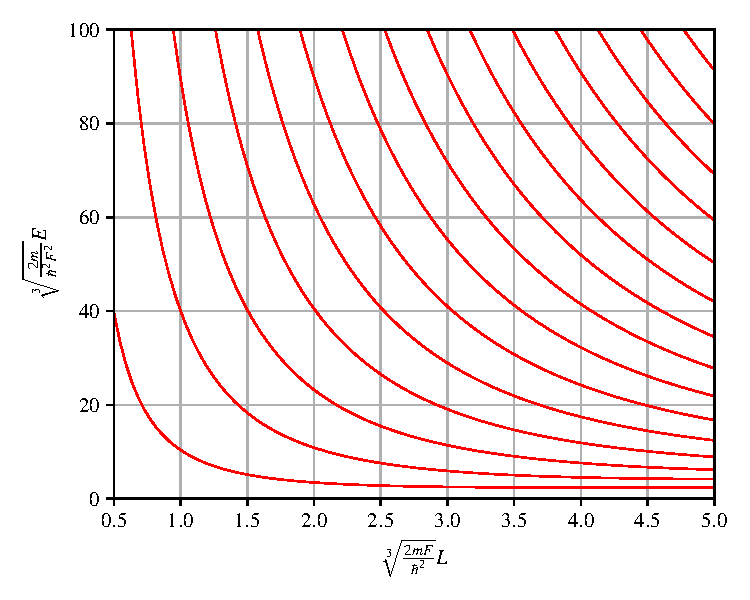
\includegraphics[scale=1]{./figs/energiaszintek.pdf}
		\caption[Egzakt energiaszintek]{Egzakt energia szintek, $bE$ és $aL$ közötti relációval ábrázolva. Az ába jobb alsó sarkán látható, hogy $E \ll FL$ esetén az energiaszintek $L$-től függetlenek lesznek, mivel a félvégtelen tér beli homogén tér energiaszintjeit közelítik.}
		\label{box_energiaszintek_abra}
	\end{figure}
	Amikor $FL \ll \frac{\pi^2\hbar^2}{2mL^2}$, a potenciál jól közelíthető konstans potenciállal, mivel az alapállapot energiájához képest is elhanyagolható a lineáris potenciál eltérése a konstans potenciáltól. Eben a esetben $E \propto n^2$. $E \ll FL$ esetben az energiaszintek jó közelítéssel konstanssá válnak. Ennek az oka, hogy $\lim_{L \to \infty}\psi(x) = \alpha \Ai\left(ax-b\right)$, mert a $\Bi\left(x\right)$ exponenciálisan növekszik nagy $x$-ek esetén. Ebben az eseten az energiaszinteket a $\Ai\left(- \sqrt[3]{\frac{2m}{\hbar^2F^2}}E\right) = 0$ egyenlet határozza meg. Ezeket az aszimptotikus viselkedéseket \aref{box_energiaszintek_abra}. ábra jól mutatja.
    
    TODO: link 1D videóról


		\subsubsection{$F=0$ eset}
			Az $F=0$ eset megoldása egyszerű, az egyik legalapvetőbb példa egyszerű kvantummechanikai rendszerekre. A sajátfüggvények
\begin{equation}
	\psi_n(x) = \sqrt{\frac{2}{L}}\sin\left(\frac{n\pi x}{L}\right),
\end{equation}
($n=1,2,\dots$), a normálási faktorok
\begin{equation}
	N_n = 1.
\end{equation}
Minden sajátfüggvény egyre normált szinusz függvény, melyek $n-1$ helyen veszik fel a $0$ értéket $x=0$ és $x=L$ között. Sajátenergiáik
\begin{equation}
	E_n = \frac{n^2\pi^2\hbar^2}{2mL^2}.
\end{equation}
Ezek az energiaszintek hasznosak lesznek a numerikus számításokban az $F\neq 0$ eseten is. 
		\subsubsection{Airy függvények}
			Az Airy egyenlet
\begin{equation}
	\frac{d^2y}{dx^2} - xy = 0,
	\label{airy:airyeq}
\end{equation}
ennek az egyenletnek a megfelelő kezdőfeltételekhez illesztett megoldásai az úgynevezett Airy-függvények, $\Ai(x)$ és $\Bi(x)$.

Az Airy-függvények szorosan kapcsolódnak a Bessel-függvényekhez. Ez elentős mind az aszimptotikus alakjuk meghatározásához, mind a függvények numerikus kiértékeléséhez. A megoldást
\begin{equation}
	y(x) = x^{\frac{1}{2}}v\left(\frac{2}{3}x^{\frac{3}{2}}\right)
\end{equation}
alakban keresve a $x \geq 0$ tartományban a $v(x)$-re vonatkozó egyenlet a módosított Bessel-egyenlet $t=\frac{2}{3}x^{\frac{3}{2}}$ bevezetésével.
\begin{equation}
	t^2\frac{d^2v(t)}{dt^2} + t\frac{dv(t)}{dt} - \left(t^2 + \frac{1}{9}\right)v(t) = 0
\end{equation}
Leolvasható, hogy $\nu^2 = \frac{1}{9}$, azaz a $v(x)$-re vonatkozó egyenlet megoldásai az $I_{\frac{1}{3}}(x)$ és $I_{-\frac{1}{3}}(x)$ módosított Bessel-függvények lineáris kombinációi.
A két hagyományosan választott lineáris kombinációk a következőek:
\begin{equation}
	\Ai(x) = \frac{\sqrt{x}}{3}\left(I_{-\frac{1}{3}}\left(\frac{2}{3}x^{\frac{3}{2}}\right)-I_{\frac{1}{3}}\left(\frac{2}{3}x^{\frac{3}{2}}\right)\right)
	\label{airy:ai+}
\end{equation}
\begin{equation}
	\Bi(x) = \sqrt{\frac{x}{3}}\left(I_{-\frac{1}{3}}\left(\frac{2}{3}x^{\frac{3}{2}}\right)+I_{\frac{1}{3}}\left(\frac{2}{3}x^{\frac{3}{2}}\right)\right).
	\label{airy:ai+}
\end{equation}
$x \leq 0$ tartományban
\begin{equation}
	y(x) = (-x)^{\frac{1}{2}}v\left(\frac{2}{3}(-x)^{\frac{3}{2}}\right)
\end{equation}
alakban keresve a megoldást a $v(x)$-re kapott egyenlet a Bessel-egyenlet, megint $\nu^2 = \frac{1}{9}$.
\begin{equation}
	t^2\frac{d^2v(t)}{dt^2} + t\frac{dv(t)}{dt} + \left(t^2 - \frac{1}{9}\right)v(t) = 0
\end{equation}
Az $x=0$ pontban megkövetelt analitikusságnak megfelelően $x \geq 0$ esetén
\begin{equation}
	\Ai(-x) = \frac{\sqrt{x}}{3}\left(J_{-\frac{1}{3}}\left(\frac{2}{3}x^{\frac{3}{2}}\right)-J_{\frac{1}{3}}\left(\frac{2}{3}x^{\frac{3}{2}}\right)\right)
	\label{airy:ai-}
\end{equation}
\begin{equation}
	\Bi(-x) = \sqrt{\frac{x}{3}}\left(J_{-\frac{1}{3}}\left(\frac{2}{3}x^{\frac{3}{2}}\right)+J_{\frac{1}{3}}\left(\frac{2}{3}x^{\frac{3}{2}}\right)\right),
	\label{airy:bi-}
\end{equation}
ahol $J_\nu(x)$ a Bessel-függvények. Érdemes definiálni a
\begin{equation}
	\Ti(x) = \frac{\Ai(x)}{\Bi(x)}
\end{equation}
függvényt.

$x \to \infty$ aszimptotikus alak:
\begin{equation}
	\Ai\left(-x\right) = \frac{1}{\sqrt{\pi}x^{1/4}}\cos\left(\frac{2}{3}x^{3/2} - \frac{\pi}{4}\right) + \mathcal{O}\left(x^{-5/4}\right)
\end{equation}
\begin{equation}
	\Bi\left(-x\right) = -\frac{1}{\sqrt{\pi}x^{1/4}}\sin\left(\frac{2}{3}x^{3/2} - \frac{\pi}{4}\right) + \mathcal{O}\left(x^{-5/4}\right)
\end{equation}
\begin{equation}
	\Ti\left(-x\right) = -\cot\left( \frac{2}{3}x^{3/2} - \frac{\pi}{4} \right) + \mathcal{O}\left(x^{-5/4}\right)
\end{equation}
\begin{equation}
	\Ai(x) = \frac{1}{2\sqrt{\pi}x^{1/4}}e^{-\frac{2}{3}x^{\frac{3}{2}}}+\mathcal{O}\left(x^{-5/4}\right)
\end{equation}
\begin{equation}
	\Bi(x) = \frac{1}{ \sqrt{\pi}x^{1/4}}e^{ \frac{2}{3}x^{\frac{3}{2}}}+\mathcal{O}\left(x^{-5/4}\right)
\end{equation}

Az állapotok normájának kiszámításához szükség van az Airy-függvények szorzatának integráljára. \cite{Albright_1977} (A.16) szerint
\begin{equation}
	\int y^2\;dx = xy^2 - {y^\prime}^2,
	\label{airy:normintegral}
\end{equation}
ahol $y$ az Airy egyenlet tetszőleges megoldása.

A Green-függvény meghatározása közben felmerül a Wronski-determinánsa az Airy-függvényeknek, ez \cite{NIST:DLMF} (9.2.7) szerint
\begin{equation}
	\mathcal{W} \{ \Ai(x), \Bi(x) \} = \Ai(x)\Bip(x) - \Bi(x)\Aip(x) = \frac{1}{\pi}
\end{equation}









		\subsubsection{Véges $F$ eset}
			Visszatérve a fizikai probléma tárgyalására \Aeqref{airy:airyeq} egyenlet \eqref{3dbox:1deq} alakúra hozható a
\begin{equation}
	x = ax^\prime - bE,
\end{equation}
\begin{equation}
	y(x) = y(ax^\prime - bE)
\end{equation}
helyettesítésekkel. A helyettesítés után $\frac{d}{dx} = \frac{1}{a}\frac{d}{dx^\prime}$, és \aeqref{airy:airyeq} alakja
\begin{equation}
	\frac{d^2y(ax^\prime-bE)}{{dx^\prime}^2} - \left(a^3x^\prime - a^2bE\right)y(ax^\prime-bE) = 0.
\end{equation}
Ezt az egyenletet összevetve \eqref{3dbox:1deq} egyenlettel $a$ és $b$ értéke leolvasható,
\begin{equation}
	\begin{aligned}
		a = \sqrt[3]{\frac{2mF}{\hbar^2}},\\
		b = \sqrt[3]{\frac{2m}{\hbar^2F^2}}.
	\end{aligned}
\end{equation}
Az egydimenziós időfüggetlen Schrödinger-egyenlet megoldása
\begin{equation}
	\psi(x) = c_1\Ai(ax-bE)+c_2\Bi(ax-bE),
\end{equation}
melyet a határfeltételekhez kell illeszteni,
\begin{equation}
	\psi(0) = \psi(L) = 0.
\end{equation}
A $\psi(0) = 0$ feltételből következik, hogy $\psi \propto \Bi(-bE)\Ai(ax-bE) - \Ai(-bE)\Bi(ax-bE)$. A második határfeltétel pedig meghatározza a lehetséges energiákat,
\begin{equation}
		0 = \psi(L) = \Bi(-bE)\Ai(aL-bE) - \Ai(-bE)\Bi(aL-bE).
		\label{vegesf:aibilevels}
\end{equation}
Felhasználva a $\Ti(x)$ függvényt, az egyenlet kompakt és jól közelíthető alakra hozható,
\begin{equation}
	\label{box_energiaszintek_egyenlet}
	\Ti(aL-bE) - \Ti(-bE) = 0.
\end{equation}
\begin{figure}[H]
	\centering
	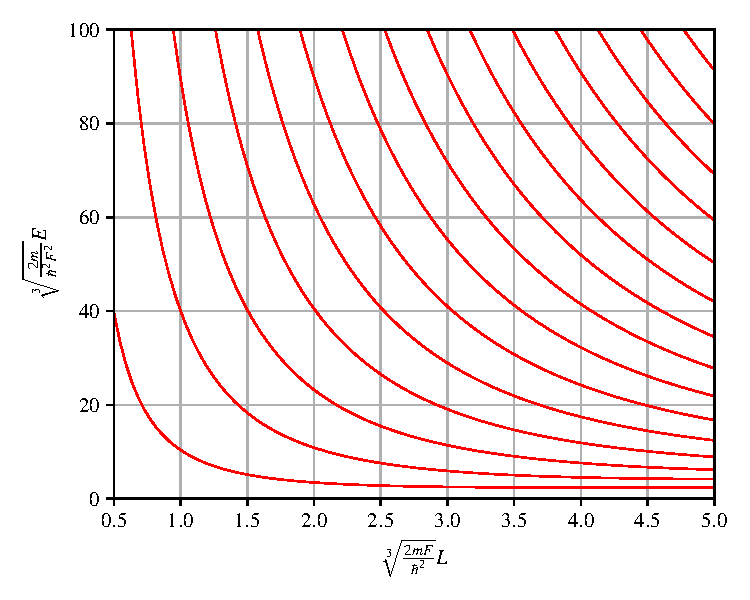
\includegraphics[scale=1]{./figs/energiaszintek.pdf}
	\caption[Egzakt energiaszintek]{Egzakt energiaszintek, $bE$ és $aL$ közötti relációval ábrázolva. Az ábra jobb alsó sarkán látható, hogy $E \ll FL$ esetén az energiaszintek $L$-től függetlenek lesznek, mivel a félvégtelen tér beli homogén tér energiaszintjeit közelítik.}
	\label{box_energiaszintek_abra}
\end{figure}
Amikor $FL \ll \frac{\pi^2\hbar^2}{2mL^2}$, a potenciál jól közelíthető konstans potenciállal, mivel az alapállapot energiájához képest is elhanyagolható a lineáris potenciál eltérése a konstans potenciáltól. Eben a esetben $E \propto n^2$. $E \ll FL$ esetben az energiaszintek jó közelítéssel konstanssá válnak. Ennek az oka, hogy $\lim_{L \to \infty}\psi(x) = \alpha \Ai\left(ax-b\right)$, mert a $\Bi\left(x\right)$ exponenciálisan növekszik nagy $x$-ek esetén. Ebben az eseten az energiaszinteket a $\Ai(-bE) = 0$ egyenlet határozza meg. Ezeket az aszimptotikus viselkedéseket \aref{box_energiaszintek_abra}. ábra jól mutatja, később a szemiklasszikus közelítés vizsgálata során részletesebben tárgyaljuk.

\begin{equation}
	\psi_k(x) = \Bi(-bE_k)\Ai(ax-bE_k) - \Ai(-bE_k)\Bi(ax-bE_k)
	\label{vegesf:psik}
\end{equation}
sajátállapotokhoz tartozó normálás analitikusan meghatározható. Mivel $\psi_k$ sajátállapotok valós értékűek, $\left|\psi_k(x)\right|^2 = \psi_k(x)^2$, így \aeqref{airy:normintegral} egyenlet közvetlenül alkalmazható,
\begin{dmath}
	N_k = \int_0^Ldx\,\left|\psi_k(x)\right|^2 = \left.\left(x-\frac{bE_k}{a}\right)\psi_k(x)^2 - \frac{1}{a^3}\psi_k^\prime(x)^2\right|_{x=0}^{x=L} = \frac{1}{a\pi^2}-\frac{1}{a}\Bigl(\Bi(-bE)\Aip(aL-bE)-\Ai(-bE)\Bip(aL-bE)\Bigr)^2.
	\label{vegesf:nk}
\end{dmath}
A $\psi_k$-t tartalmazó tagok kiesnek a határokon, mert a határfeltételeknek megfelelően $\psi_k=0$ $x=0$ és $x=L$-ben. A maradéktag $x=0$-beli értéke $\frac{1}{\pi^2}$ az Airy-függvények Wronski-determinánsa \eqref{airy:wronski} miatt. \Aref{vegesf:eigenstates}. ábra az első néhány sajátállapotot szemlélteti,  $1$-re normálva az $N_k$ együtthatók segítségével.
\begin{figure}[H]
	\centering
	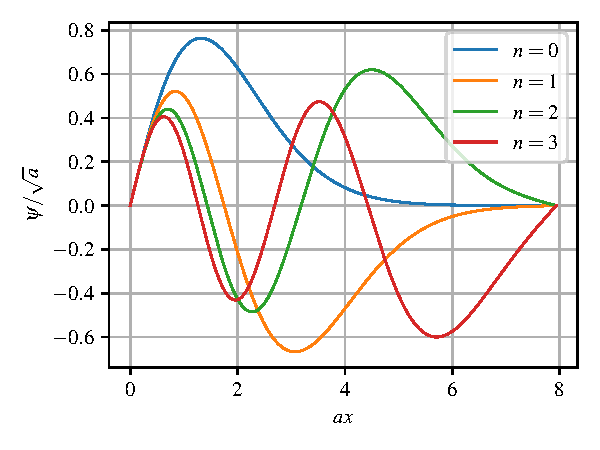
\includegraphics[scale=1]{./figs/allapotok.pdf}
	\caption[Sajátállapotok]{Az első $4$ energia sajátállapot $aL=8$ hosszúságú doboz esetén, $1$-re normálva, azaz $\frac{1}{\sqrt{N_n}}\psi_n(x)$ függvényeket ábrázolva ($n=0,1,2,3$).}
	\label{vegesf:eigenstates}
\end{figure}
	
%A probléma egy 1D dobozba zárt résecske homogén erőtérben. $F(x)=-F$, azaz $V(x) = Fx$.
%	Az egyenlethez tartozó határfeltételek, ha a doboz hossza $L$:
%	\begin{equation}
%		\phi \big\rvert_0 = \phi \big \rvert_L = 0
%	\end{equation}
%	A megoldandó időfüggetlen Schrödinger-egyenlet:
%	\begin{equation}
%		-\frac{\hbar^2}{2m}\frac{d^2\phi}{dx^2} + Fx\phi = E\phi
%	\end{equation}
%	\begin{equation}
%		\frac{d^2\phi}{dx^2} - \frac{2mFx}{\hbar^2}\phi = -\frac{2mE}{\hbar^2}\phi
%	\end{equation}
%	\begin{equation}
%		\frac{d^2\phi}{dx^2} - \left(\frac{2mF}{\hbar^2}x - \frac{2mE}{\hbar^2}\right)\phi = 0
%	\end{equation}
%	Az Airy egyenlet ilyen alakra hozható a változó affin lineáris transzformációjával:
%	\begin{equation}
%		\frac{d^2y}{dx^{\prime 2}} - x^\prime y = 0
%	\end{equation}
%	$x^\prime = ax - bE$, azaz $\frac{d}{dx} = a\frac{d}{dx^\prime}$:
%	\begin{equation}
%		\frac{d^2y}{dx^2} - \left(a^3x - a^2bE\right)y = 0
%	\end{equation}
%	Az együtthatók összevetése alapján $a = \sqrt[3]{\frac{2mF}{\hbar^2}}$ és $b = \sqrt[3]{\frac{2m}{\hbar^2F^2}}$. Így a Schrödinger-egyenlet megoldása:
%	\begin{equation}
%		\phi(x) = y(x^\prime) = y\left(\sqrt[3]{\frac{2mF}{\hbar^2}}x - \sqrt[3]{\frac{2m}{\hbar^2F^2}}E\right)
%	\end{equation}
%	, ahol $y(x) = \alpha \Ai\left(x\right) + \beta \Bi\left(x\right)$.
%	A $\phi \big\rvert_0 = 0$ feltételből következik, hogy $\phi \propto \Bi\left(-bE\right)\Ai\left(ax-bE\right) - \Ai\left(-bE\right)\Bi\left(ax-bE\right)$. A második határfeltétel pedig meghatározza a lehetséges energiákat. A feltétel:
%	\begin{equation}
%		\Bi\left(-bE\right)\Ai\left(aL-bE\right) - \Ai\left(-bE\right)\Bi\left(aL-bE\right) = 0
%	\end{equation}
%	\begin{equation}
%		\label{box_energiaszintek_egyenlet}
%		\Ti{aL-bE} - \Ti{-bE} = 0
%	\end{equation}
%	\begin{equation}
%		\Ti{\sqrt[3]{\frac{2mF}{\hbar^2}}L - \sqrt[3]{\frac{2m}{\hbar^2F^2}}E} - \Ti{-\sqrt[3]{\frac{2m}{\hbar^2F^2}}E} = 0
%	\end{equation}
%	\begin{figure}[H]
%		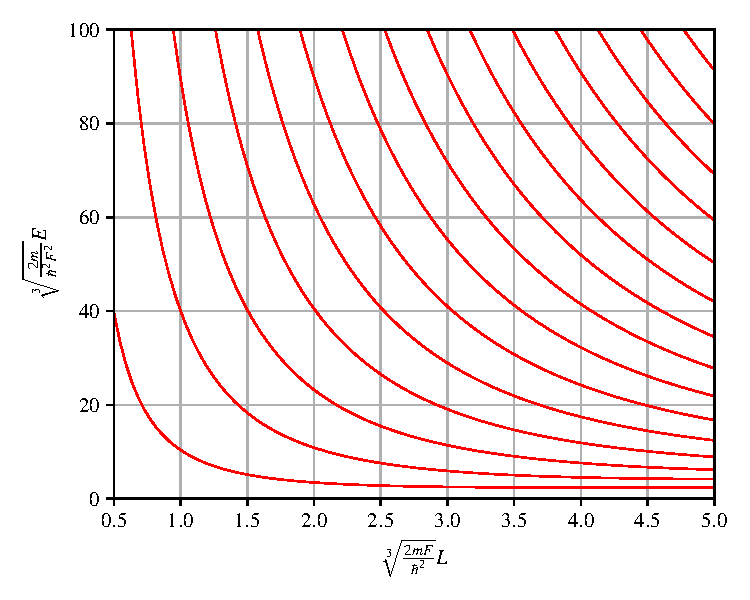
\includegraphics[scale=1]{./figs/energiaszintek.pdf}
%		\caption[Egzakt energiaszintek]{Egzakt energia szintek, $bE$ és $aL$ közötti relációval ábrázolva. Az ába jobb alsó sarkán látható, hogy $E \ll FL$ esetén az energiaszintek $L$-től függetlenek lesznek, mivel a félvégtelen tér beli homogén tér energiaszintjeit közelítik.}
%		\label{box_energiaszintek_abra}
%	\end{figure}
%	Amikor $FL \ll \frac{\pi^2\hbar^2}{2mL^2}$, a potenciál jól közelíthető konstans potenciállal, mivel az alapállapot energiájához képest is elhanyagolható a lineáris potenciál eltérése a konstans potenciáltól. Eben a esetben $E \propto n^2$. $E \ll FL$ esetben az energiaszintek jó közelítéssel konstanssá válnak. Ennek az oka, hogy $\lim_{L \to \infty}\psi(x) = \alpha \Ai\left(ax-b\right)$, mert a $\Bi\left(x\right)$ exponenciálisan növekszik nagy $x$-ek esetén. Ebben az eseten az energiaszinteket a $\Ai\left(- \sqrt[3]{\frac{2m}{\hbar^2F^2}}E\right) = 0$ egyenlet határozza meg. Ezeket az aszimptotikus viselkedéseket \aref{box_energiaszintek_abra}. ábra jól mutatja.
%    
%    TODO: link 1D videóról
%
		\subsubsection{Falak nélküli eset}
			Falak hiányában a Schrödinger-egyenlet továbbra is \eqref{3dbox:1deq}, azonban a határfeltételek különböznek. A fizikai kép az, hogy $V(x)=Fx$ potenciál esetén az $x\to\infty$-ből nem jönnek részecskék, és nem is tartózkodnak ott. Ezek problémás állapotok lennének, végtelen energiával rendelkeznének. Tehát a szórásállapotokra vonatkozó feltétel, hogy
\begin{equation}
	\lim_{x\to\infty}\psi(x) = 0.
	\label{nowall:oundary}
\end{equation}
Mivel itt folytonos spektrumról van szó, az eddigi normálás helyett az állapotokat Dirac-deltára kell normálni. Ebben a feladatban az energia és energia sajátállapot között egy az egyhez megfeleltetés van, ellenben a jól ismert szabad részecske esetével. Ennek oka, hogy itt $x\to\infty$-ből nem jönnek részecskék. Ennek következtében az a sajátállapotokat $\Ket{E}$ egyértelmen jelöli.
\Aeqref{nowall:oundary} feltétel azt jelenti, hogy az Airy-függvények közül a $\Bi(ax-bE)$ nem szerepel a lineáris kominációban, a megoldás tisztán az $\Ai(ax-bE)$ függvény lesz,
\begin{equation}
	\Braket{x|E}=N\Ai(ax-bE).
\end{equation}
A szórásállapotokra vonatkozó normálási feltétel
\begin{equation}
	\Braket{E|E^\prime}=\delta(E-E^\prime).
\end{equation}
Ez alapján $N$ meghatározható \eqref{airy:delta} azonosság felhasználásával,
\begin{dmath}
	\delta(E-E^\prime)=N^2\int_{-\infty}^\infty\Ai(ax-bE)\Ai(ax-bE^\prime)\,dx=N^2\frac{1}{ab}\delta(E-E^\prime).
\end{dmath}
Ez alapján $N=\sqrt{ab}=\sqrt[3]{\frac{2m}{\hbar^2\sqrt{F}}}$, és
\begin{equation}
	\Braket{x|E}=\psi_E(x)=\sqrt{ab}\Ai(ax-bE).
\end{equation}
A teljességi reláció is leellenőrizhető \aeqref{airy:delta} egyenlet alapján,
\begin{dmath}
	\int_{-\infty}^\infty dE\,\Ket{E}\Bra{E}=ab\int_{-\infty}^\infty dE\int_{-\infty}^\infty dx\int_{-\infty}^\infty dy\,\Ai(ax-bE)\Ai(ay-bE)\Ket{x}\Bra{y}=\int_{-\infty}^\infty dx\int_{-\infty}^\infty dy\,\delta(x-y)\Ket{x}\Bra{y}=\op{I}.
\end{dmath}
\section{Szemiklasszikus közelítés}
	\begin{equation}
		nh = \oint p \, dq = 
	\end{equation}
	$E/F < L$ esete:
	\begin{equation}
		2\int_0^{E/F}\sqrt{2m\left( E-Fx \right)}\,dx = -\frac{2}{3mF}\left(2m\left( E-Fx \right)\right)^{\frac{3}{2}}\bigg \rvert_0^{E/F} = \frac{4\sqrt{2m}E^{3/2}}{3F}
	\end{equation}
	\begin{equation}
		E_n = \left(\frac{3nhF}{4\sqrt{2m}}\right)^{2/3}
	\end{equation}
	$E/F > L$ esete:
	\begin{equation}
		-\frac{2}{3mF}\left(2m\left( E-Fx \right)\right)^{\frac{3}{2}}\bigg \rvert_0^{L} = \frac{4\sqrt{2m}}{3F}\left(E^{3/2} - \left(E - FL\right)^{3/2}\right) = nh
	\end{equation}
	$E \gg FL$ esetén a különbség az $E^{3/2}$ függvény deriváltjának segítségével helyettesíthető:
	\begin{equation}
		nh \approx 2\sqrt{2m}E^{1/2}L
	\end{equation}
	\begin{equation}
		E_n \approx \frac{n^2h^2}{8mL^2}
	\end{equation}
	
	\begin{figure}[H]
		\centering
		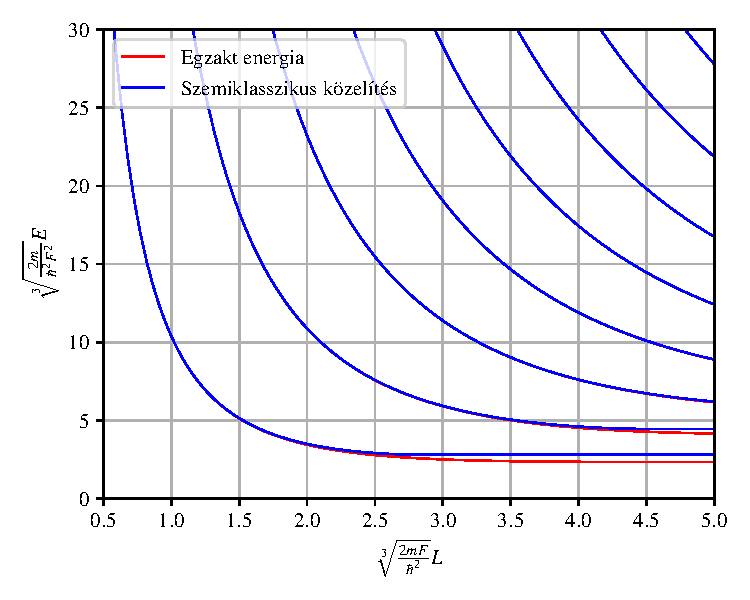
\includegraphics[scale=1]{./figs/energiaszintkozelites.pdf}
		\caption[Szemiklasszikus energiaszintek]{Az ábra a szemiklasszikus energiaszinteket hasonlítja össze az egzakt energiaszintekkel. Ez az ábra is a $bE$ és $aL$ közötti relációt ábrázolja. A szemiklasszikus közelítés nagy kvantumszámok illetve $E \gg FL$ esetén pontos. Utóbbi oka, hogy ebben az esetben a potenciál elhanyagolható, és a potenciál nélküli végtelen potenciálgödör energiaszintjeit pedig a szemiklasszikus közelítés egzaktul megadja.}
	\end{figure}
	
	\begin{figure}[H]
		\centering
		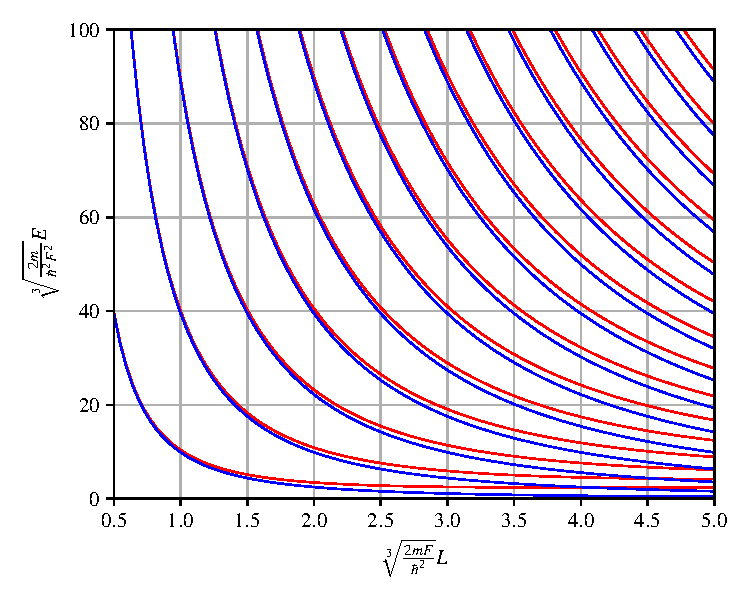
\includegraphics[scale=1]{./figs/infsquareenergia.pdf}
		\caption[Végtelen potenciálgödör energiaszintjei]{Az ábrán a végtelen potenciálgödör és az egzakt energiaszintek összehasonlítása látható. Ez csak az $E \gg FL$ esetben jó közelítés, a szemiklasszikus energiaszintek jóval pontosabbak.}
	\end{figure}


	\subsection{Szemiklasszikus energiaszintek}
		A dobozba zárt részecske esetében két esetet kell vizsgálni a szemiklasszikus energiaszintek meghatározásához. Az első eset, amikor az energia $E < FL$, tehát a fordulópont a második fal elérése előtt van. Ebben az esetben a Maslov index $\frac{3}{4}$ \cite{brack:semiclassical} (2.4.1 fejezet). Az $x=0$ fordulópontban a szemiklasszikus hullámfüggvény $\frac{\pi}{4}$ fázist vesz fel, az $x=E/F$ fordulópontban pedig $\frac{\pi}{2}$ fázist vesz fel,
\begin{equation}
	\left(n+\frac{3}{4}\right)h=\oint p\,dq=2\int_0^{E/F}\sqrt{2m\left( E-Fx \right)}\,dx=\frac{4\sqrt{2m}}{3F}E^{3/2}.
	\label{semiclassicallevels:e1}
\end{equation}
A második eset amikor $E > FL$, ekkor a fordulópontok $0$-ban és $L$-ben vannak, és a Maslov index $1$. Mind az $x=0$, mind az $x=L$ fordulópontban $\frac{\pi}{2}$ fázis vesz fel a szemiklasszikus hullámfüggvény,
\begin{equation}
	\left(n+1\right)h=\oint p\,dq=2\int_0^{L}\sqrt{2m\left(E-Fx\right)}\,dx=\frac{4\sqrt{2m}}{3F}\left(E^{3/2}-\left(E-FL\right)^{3/2}\right).
	\label{semiclassicallevels:e2}
\end{equation}
Előfordulhat, hogy valamely $n$-re egyszerre van \eqref{semiclassicallevels:e1} és \eqref{semiclassicallevels:e2} egyszerre van megoldása, ahol $E$ a megfelelő tartományba esik. Ez azt jelenti, hogy a szemiklasszikus közelítés hibáján belül nem lehet meghatározni, hogy a valódi energiszint $FL$ felett, vagy alatt van. \Aref{semiclassicallevels:allapotszam}. ábra szemlélteti a szemiklasszikus és egzakt állapotszámok viszonyát.
\begin{figure}[H]
	\centering
	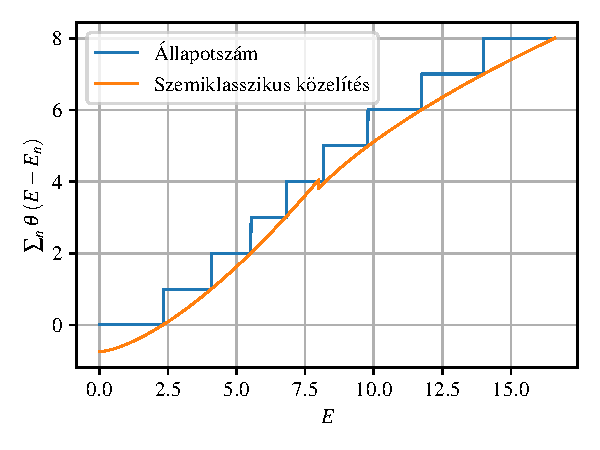
\includegraphics[scale=1]{./figs/allapotszam.pdf}
	\caption[Szemiklasszikus állapotszám]{A szemiklasszikus és egzakt energiaszintek összevetése. A kék vonal az egzakt energiák által meghatározott állapotszám. A narancssárga vonal pedig \aeqref{semiclassicallevels:e1} és \aeqref{semiclassicallevels:e2} egyenletekből kifejezett $n$ az energia függvényében, $E$ és $FL$ relációjának megfelelően.}
	\label{semiclassicallevels:allapotszam}
\end{figure}
\begin{figure}[H]
	\centering
	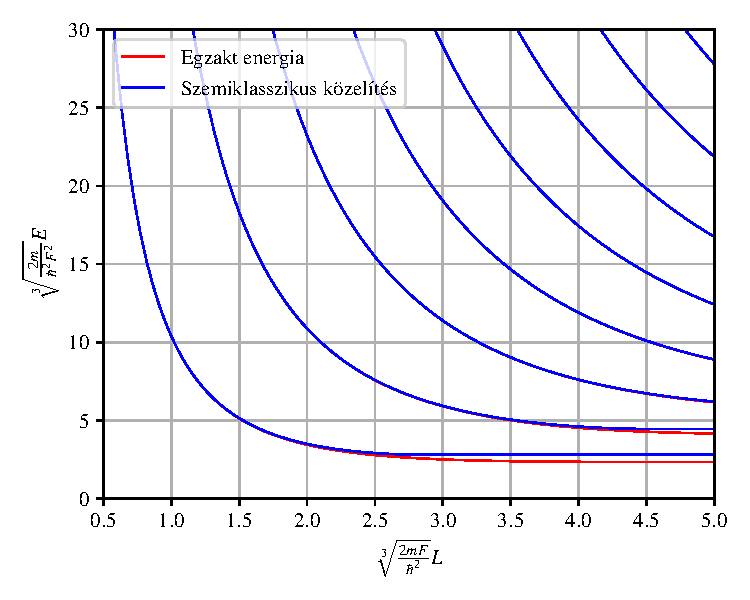
\includegraphics[scale=1]{./figs/energiaszintkozelites.pdf}
	\caption[Szemiklasszikus energiaszintek]{Az ábra a szemiklasszikus energiaszinteket hasonlítja össze az egzakt energiaszintekkel. Ez az ábra is a $bE$ és $aL$ közötti relációt ábrázolja. A szemiklasszikus közelítés nagy kvantumszámok illetve $E \gg FL$ esetén pontos. Utóbbi oka, hogy ebben az esetben a potenciál elhanyagolható, és a potenciál nélküli végtelen potenciálgödör energiaszintjeit pedig a szemiklasszikus közelítés egzaktul megadja.}
	\label{semiclassicallevels:kozelites}
\end{figure}
\begin{figure}[H]
	\centering
	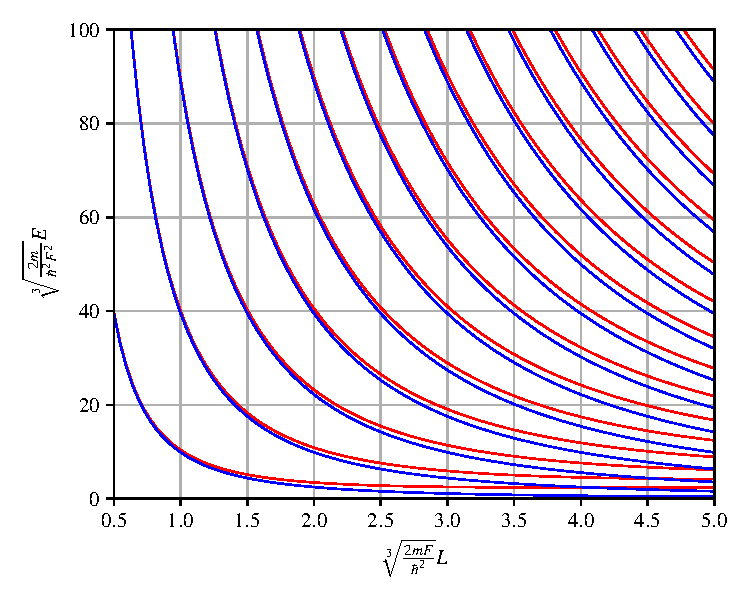
\includegraphics[scale=1]{./figs/infsquareenergia.pdf}
	\caption[Végtelen potenciálgödör energiaszintjei]{Az ábrán a végtelen potenciálgödör és az egzakt energiaszintek összehasonlítása látható. Ez csak az $E \gg FL$ esetben jó közelítés, a szemiklasszikus energiaszintek jóval pontosabbak.}
	\label{semiclassicallevels:squarewell}
\end{figure}
	\subsection{Összehasonlítás az egzakt eredménnyel}
		\Aeqref{box_energiaszintek_egyenlet} egyenletet nagy $bE$ illetve nagy $bE-aL$ esetén \aeqref{airy:tiapprox} közelítés alkalmazható,
\begin{equation}
	\ctg\left(\frac{2}{3}\left(bE-aL\right)^{3/2}-\frac{\pi}{4}\right)-\ctg\left(\frac{2}{3}\left(bE\right)^{3/2}-\frac{\pi}{4}\right)=0.
	\label{quantumApprox:cot}
\end{equation}
A $\ctg(x)$ függvény $\pi$-ben periodikus, és mivel a $(0,\pi)$ intervallumban szigorúan monoton csökken, \aeqref{quantumApprox:cot} egyenletnek csak akkor van megoldása, ha a $\ctg(x)$ függvények argumentumainak különbsége $n\pi$, azaz
\begin{equation}
	\frac{2}{3}\left(bE\right)^{3/2}-\frac{2}{3}\left(bE-aL\right)^{3/2}=n\pi.
\end{equation}
Az $a$ és $b$ állandók behelyettesítésével ez az egyenlet \aeqref{semiclassicallevels:e2} egyenletet adja. Az $n$  értéke ugyan különbözik $1$-gyel a két egyenletben a Maslov indexek miatt, viszont mivel $n$ egész, ugyan azokat az energiaszinteket határozzák meg. Ennek nem feltétlenül kéne így lennie, viszont ebben az esetben a szemiklasszikus illetve az Airy-függvények aszimptotikus alakjából kapott közelítések egzaktul megegyeznek.

Amennyiben $bE-aL$ negatív, a $\Ti(bE-aL)$ gyorsan lecseng, \aeqref{quantumApprox:cot} egyenlet bal oldalának első tagja elhanyagolható. Ennek a tagnak az elhanyagolásával \aeqref{semiclassicallevels:e1} egyenletet kapjuk vissza. Ez a képlet felel meg az $L\to\infty$ határesetnek, ami a féltérben pattogó labdát írja le.

%$x \to \infty$ aszimptotikus alak:
%	\begin{equation}
%		\Ai\left(-x\right) = \frac{1}{\sqrt{\pi}x^{1/4}}\cos\left(\frac{2}{3}x^{3/2} - \frac{\pi}{4}\right) + \mathcal{O}\left(x^{-5/4}\right)
%	\end{equation}
%	\begin{equation}
%		\Bi\left(-x\right) = -\frac{1}{\sqrt{\pi}x^{1/4}}\sin\left(\frac{2}{3}x^{3/2} - \frac{\pi}{4}\right) + \mathcal{O}\left(x^{-5/4}\right)
%	\end{equation}
%	\begin{equation}
%		\Ti\left(-x\right) = -\cot\left( \frac{2}{3}x^{3/2} - \frac{\pi}{4} \right) + \mathcal{O}\left(x^{-5/4}\right)
%	\end{equation}
%	
%	Ezzel a közelítéssel \aref{box_energiaszintek_egyenlet}. egyenlet alakja:
%	\begin{equation}
%		\cot\left(\frac{2}{3}\left(bE-aL\right)^{3/2} - \frac{\pi}{4}\right) = \cot\left(\frac{2}{3}\left(bE\right)^{3/2} - \frac{\pi}{4}\right)
%	\end{equation}
%	, azaz
%	\begin{equation}
%		\frac{2}{3}\left(bE\right)^{3/2} - \frac{2}{3}\left(bE-aL\right)^{3/2} = n\pi
%	\end{equation}
%	. Az $a$ és $b$ behelyettesítésével az egyenlet
%	\begin{equation}
%		\frac{2\sqrt{2m}}{3F\hbar}\left(E^{3/2} - \left(E - FL\right)^{3/2}\right) = n\pi
%	\end{equation}
%	Ez megegyezik a szemiklasszikus kvantálással kapott eredménnyel, ami azt jelenti, hogy a szemiklasszikus közelítés jól működik nagy energiáknál, hibája $\mathcal{O}\left(E^{-5/4}\right)$ nagyságrendű.


	\subsection{Airy függvények aszimptotikája}
		Klasszikus mechanikai megfontolások alapján meghatározhatóak az Airy-függvények aszimptotikus alakjai, a pontos fázistól eltekintve. Ez nem meglepő, mert a hullámfüggvény amplitúdója a megtalálási valószínűséggel van kapcsolatban. A hullámfüggvény lokális közelítése egy síkhullámmal, vagyis a fázis deriváltja az impulzussal van kapcsolatban. Így a klasszikus mechanika alapján lehet a hullámfüggvény amplitúdójára és fázisára következtetni.

\Aref{nowall}. fejezetben leírt rendszert vizsgáljuk, $E=0$ választásával, azaz a klasszikus esetben a fordulópont $x=0$-ban van. Kvantum mechanika szerint a megtalálási valószínűség $|\psi|$-tel arányos, klasszikus mechanikában pedig a $dx$ tartományon való áthaladás idejével, $\frac{dx}{v}$-vel arányos. Mivel a kérdéses állapot szórásállapot, nem normálható. Ezért a valószínűségeknél csak arányosságról beszélhetünk, egy részecske rendszerre vonatkozó valószínűségsűrűségként nem értelmezhető. Egy lehetséges interpretáció a szórásállapotok esetében $|\psi|^2$-re, hogy nem kölcsönható részecske áramról van szó, és a résecskék sűrűsége $|\psi|^2$-tel arányos. A klasszikus esetben hasonló a helyzet, a $\frac{dx}{v}$ a részecskesűrűséggel arányos. A két módon kapott részecskesűrűség egyenlőségének feltételezésével a hullámfüggvény amplitúdójának viselkedését kapjuk,
\begin{equation}
	\frac{dx}{v}=\sqrt{-\frac{m}{2Fx}}dx\propto \lvert\psi(x)\rvert^2dx,
\end{equation}
a klasszikus mechanikából ismert energia megmaradás szerint. Átrendezve
\begin{equation}
	\psi(x)\propto\frac{1}{\sqrt[4]{-x}}.
\end{equation}
A hullámfüggvény fázisának meghatározása a de Broglie hullámhossz, $p=\hbar k$, és a klasszikus impulzus alapján történik. Abban az esetben, ha az amplitúdó ami közelítőleg megkapható az előző egyenletből, kicsit változik a de Broglie hullámhossz alatt,
\begin{equation}
	\psi(x)\propto\exp\left(\pm i\int_{x_0}^xk\left(x^\prime\right)\,dx^\prime\right),
	\label{asymtotics:phase}
\end{equation}
Attól függően, hogy a részecske $+x$ vagy $-x$ irányban halad. A klasszikus energia megmaradás meghatározza az impulzust, ami alapján a de Broglie hullámszám
\begin{equation}
	k=\frac{\sqrt{2mF}}{\hbar}\sqrt{-x}.
\end{equation}
A $k$ integrálja könnyen kiszámítható,
\begin{equation}
	\int \frac{\sqrt{2mF}}{\hbar}\sqrt{-x}\,dx=\frac{2}{3}\left(-ax\right)^{3/2}.
\end{equation}
A részecskeáram klasszikusan mindenhol $0$, ebben a potenciálban minden részecske visszaesik. Ez a feltétel ekvivalens azzal a feltétellel, hogy $\psi$ valós, azaz \aeqref{asymtotics:phase} egyenletnek csak bizonyos kombinációi léphetnek fel. Ezt írja le az exponenciális függvény helyettesítése a szinusz függvénnyel, és a $\phi_0$ fázistolás,
\begin{equation}
	\psi(x)\propto\Ai(ax)\approx\frac{1}{\sqrt[4]{-ax}}\sin\left(\frac{2}{3}\left(-ax\right)^{3/2}+\phi_0\right).
\end{equation}
Ez az egyenlet kombinálja a fázisra és az amplitúdóra vonatkozó feltételeket, és egyezik \aeqref{airy:ai-approx} és \aeqref{airy:bi-approx} aszimptotikus alakokkal.

Pozitív $x$ esetén a kinetikus energia negatív lenne, ami formálisan képzetes de Broglie hullámhossznak felel meg. Ezen formális összefüggés alapján az aszimptotikus alakot az amplitúdó járulékát leszámítva ($\frac{1}{\sqrt[4]{x}}$ tényező) pusztán fizikai meggondolások alapján megkappjuk,
\begin{equation}
	\Ai(x)\approx\exp\left(-\frac{2}{3}x^{3/2}\right).
\end{equation}
Érdemes megjegyezni, hogy az ellentétes előjelű komplex hullámhossz a $\Bi$ aszimptotikus alakjához tartozik,
\begin{equation}
	\Bi(x)\approx\exp\left(\frac{2}{3}x^{3/2}\right).
\end{equation}
A $\frac{1}{\sqrt[4]{x}}$ részt leszámítva ez egyezik \aeqref{airy:ai+approx} és \aeqref{airy:bi+approx} egyenletekkel, az aszimptotika exponenciális részét helyesen megkaptuk.



\section{Homogén tér Green-függvénye}
	A reolvens operátor definíciója
\begin{equation}
    \op{G}\left( E \right) = \frac{1}{\op{H} - E}
\end{equation}
és ezen operátorhoz tartozó két változós függvény a Green-függény.
\begin{equation}
    G\left( x, y; E \right) = \Bra{x}G\left(E\right)\Ket{y}
\end{equation}
A Green-függvény név indokolt, és ennek a segítségével fogom meghatározni a Green-függvényeket konkrét esetben. A teljességi reláció beszúrásával látható, hogy a kvantummechanikai Green-függény megegyezik a differenciálegyenletek elméletéből ismert Green-függvénnyel.
\begin{equation}
    \left(\op{H} - E\right) \op{G}\left( E \right) = \op{I}
\end{equation}

\begin{equation}
    \int \mathrm{d}x^\prime \Bra{x}\left(\op{H} - E\right) \Ket{x^\prime}\Bra{x^\prime} \op{G}\left( E \right)\Ket{y} = \Bra{x}\op{I}\Ket{y} = \delta \left(x - y\right)
\end{equation} 
A $\Bra{x}\left(\op{H} - E\right) \Ket{x^\prime}$ maggal vett konvolúció a $\op{H} - E$ operátor hatása. Ezért
\begin{equation}
    \left(\op{H}_x - E\right) G\left(x, y; E\right) = \delta\left(x - y\right)
\end{equation}
ami a differenciálegyenletek elméletéből ismert Green-függvény definíciója. Ebben a konkrét esetben
\begin{equation}
    \left( -\frac{\hbar^2}{2m}\frac{\partial^2}{\partial x^2} + Fx - E \right) G\left(x, y; E\right) = \delta\left(x - y\right)
	\label{green:deltaeq}
\end{equation}
\subsection{Egzakt Green-függvény}
ami azt jelenti, hogy az $x < y$ tartományban
\begin{equation}
    G\left(x, y; E\right) = C_1 \Ai{\sqrt[3]{\frac{2mF}{\hbar^2}}x - \sqrt[3]{\frac{2m}{\hbar^2F^2}}E} + C_2 \Bi{\sqrt[3]{\frac{2mF}{\hbar^2}}x - \sqrt[3]{\frac{2m}{\hbar^2F^2}}E}
    \label{green:xy}
\end{equation}
illetve az $x > y$ tartományban
\begin{equation}
    G\left(x, y; E\right) = C_3 \Ai{\sqrt[3]{\frac{2mF}{\hbar^2}}x - \sqrt[3]{\frac{2m}{\hbar^2F^2}}E} + C_4 \Bi{\sqrt[3]{\frac{2mF}{\hbar^2}}x - \sqrt[3]{\frac{2m}{\hbar^2F^2}}E}
    \label{green:yx}
\end{equation}
, ahol a $C$ együtthatók függhetnek $y$ és $E$ értékétől. A $C$ együtthatók meghatározásához a doboz eredeti határfeltételeit $x = 0$ és $x = L$ pontban, valamint az $x = y$ pontban \aref{green:deltaeq}. egyenlet $y$ körüli integrálásából kapot feltételeket kell felhasználni. A doboz falára vonatkozó határfeltételek:
\begin{equation}
	\left. G\left(x,y;E\right)\right\rvert_{x = 0} = 0
\end{equation}
\begin{equation}
	\left. G\left(x,y;E\right)\right\rvert_{x = L} = 0
\end{equation}
\Aref{green:deltaeq}. egyenlet $\int_{y-\epsilon}^{y+\epsilon}\mathrm{d}x^\prime \int_{y}^{x^\prime} \mathrm{d}x$ szerinti integrálja az $\epsilon \to 0^+$ határesetben: 
\begin{equation}
	\lim_{\epsilon \to 0^+}\left.G\left(x,y;E \right)\right\rvert_{x = y - \epsilon}^{x = y + \epsilon} = 0
\end{equation}
A jobb oldal integrálja $\left. \left(x - y\right) \theta\left(x - y\right) \right\rvert_{x=y-\epsilon}^{x=y+\epsilon}$, ami a határesetben $0$. Az $\left(Fx - E\right)G\left(x,y;E\right)$ integrálja is $0$ a határesetben, mert az erdeti függvény is folytonos, így az integrálja is. \Aref{green:deltaeq}. egyenlet $x$ szerinti integrálja $y$ körüli $\epsilon$ sugarú környezetében az $\epsilon \to 0^+$ határesetben:
\begin{equation}
	\lim_{\epsilon \to 0^+}\left.\frac{\partial}{\partial x}G\left(x,y;E \right)\right\rvert_{x = y - \epsilon}^{x = y + \epsilon} = -\frac{2m}{\hbar^2}
\end{equation}
Itt a jobb oldal integrálja $\left. \theta\left(x - y\right) \right\rvert_{x = y - \epsilon}^{x = y + \epsilon} = 1$ a határesetben. A bal oldalon az előzőhöz hasonló módon csak a derivált integrálja marad meg. \Aref{green:xy}. és \aref{green:yx}. egyenlet behelyettesítése meghatározza a $C$ együtthatókra vonatkozó egyenleteket:
\begin{equation}
	\frac{C_2}{C_1} = -\Ti{-bE}
	\label{green:Cbegin}
\end{equation}
\begin{equation}
	\frac{C_4}{C_3} = -\Ti{b\left(FL - E\right)}
\end{equation}
\begin{equation}
	\frac{C_3}{C_1} = \frac{\Ti{ay - bE} + \Ti{-bE}}{\Ti{ay - bE} + \Ti{b\left(FL - E\right)}}
\end{equation}
TODO: $b$ lecserélése $bE$-re az előző részekben.
\begin{equation}
	C_1 = -\frac{2m}{a\hbar^2}\frac{1}{\left( \left(\frac{C_3}{C_1}-1\right)\Aip{ay - bE} + \left(\frac{C_4}{C_3}\frac{C_3}{C_1} - \frac{C_2}{C_1}\right) \Bip{ay - bE} \right)}
	\label{green:Cend}
\end{equation}
\begin{equation}
	C_1 = -\frac{a^2}{F}\frac{1}{\left( \left(\frac{C_3}{C_1}-1\right)\Aip{ay - bE} + \left(\frac{C_4}{C_3}\frac{C_3}{C_1} - \frac{C_2}{C_1}\right) \Bip{ay - bE} \right)}
\end{equation}
\Aref{green:Cbegin}-\ref{green:Cend}, \ref{green:xy}. és \aref{green:yx}. egyenletek explicit, analitikus módon előállítják a $G\left( x, y; E \right)$ Green-függvényt.
\subsection{Green-függvény perturbáció számítással}
A perturbációszámításhoz a Hamilton operátort két részre bontom fel:
\begin{equation}
	\op{H} = \op{H}_0 + \op{V}
\end{equation}
A $\op{H}_0$ operátorhoz tartozó rezolvens $\op{G}_0\left(E\right)$. $\op{H}$ és $\op{H}_0$ kifejezhetőek a rezolvenseikkel. Ha a kifejezéseket behelyettesítjük a fenti egyenletbe, implicit egyenletet kapunk $op{G}\left(E\right)$-re nézve, melyet fel lehet használni perturbációszámításra. Az egyenletet balról $\op{G}_0^{-1}\left(E\right)$-vel, jobbról $\op{G}^{-1}\left(E\right)$-vel szorzunk.
\begin{equation}
	\op{G}^{-1}\left(E\right) + E = \op{G}_0^{-1}\left(E\right) + E + \op{V}
\end{equation}
\begin{equation}
	\op{G}\left(E\right) = \op{G}_0\left(E\right) - \op{G}_0\left(E\right)\op{V}\op{G}\left(E\right)
	\label{green:pertmaster}
\end{equation}
Az alábbi módon definiálva $\op{G}_n\left(E\right)$ operátort, \aref{green:pertmaster}. egyenlethez hasonló rekurziós összefüggés áll fent:
\begin{equation}
	\op{G}_n\left(E\right) = \op{G}_0\left(E\right)\sum_{k=0}^n\left(-\op{V}\op{G}_0\left(E\right)\right)^k
\end{equation}
\begin{equation}
	\op{G}_{n+1}\left(E\right) = \op{G}_0\left(E\right) - \op{G}_0\left(E\right)\op{V}\op{G}_n\left(E\right)
\end{equation}
Ha $\norm{\op{V}\op{G}_0\left(E\right)} < 1$ akkor a $\op{G}_n$ sorozat konvergál, és kielégíti \aref{green:pertmaster}. egyenletet. Ezért konvergencia esetén:
\begin{equation}
	\op{G}\left(E\right) = \op{G}_0\left(E\right)\sum_{n=0}^\infty\left(-\op{V}\op{G}_0\left(E\right)\right)^n
\end{equation}
A perturbbálatlan operátornak a lineáris potenciál nélküli dobozba zárt részecske Hamilton operátorát választom, $\op{H}_0=\frac{1}{2m}\op{p}^2$, így a lineáris potenciál marad a perturbáció $\op{V} = F\op{x}$. A perturbálatlan $\op{G}_0\left(E\right)$ Green-függvényt is \aref{green:Cbegin}-\ref{green:Cend}, \ref{green:xy}. és \aref{green:yx}. egyenletek alapján határozom meg.
\begin{equation}
	G_0\left(x,y;E\right) =
	\begin{cases}
		-\frac{2m}{k\hbar^2}\frac{1}{\sin\left(kL\right)} \sin\left(k\left(y-L\right)\right)\sin\left(kx\right) & x\leq y\\
		-\frac{2m}{k\hbar^2}\frac{1}{\sin\left(kL\right)} \sin\left(k\left(x-L\right)\right)\sin\left(ky\right) & x>y\\
	\end{cases}
\end{equation}







	\subsection{Egzakt Green-függvény}
		A Green-függvény név indokolt: a teljességi reláció beszúrásával látható, hogy a kvantummechanikai Green-függény megegyezik a differenciálegyenletek elméletéből ismert Green-függvénnyel.
\begin{equation}
    \left(E-\op{H}\right)\op{G}\left( E \right) = \op{I},
\end{equation}
azaz
\begin{equation}
    \int dx^\prime \Bra{x}\left(E-\op{H}\right) \Ket{x^\prime}\Bra{x^\prime} \op{G}\left( E \right)\Ket{y} = \Bra{x}\op{I}\Ket{y} = \delta \left(x - y\right).
\end{equation} 
A $\Bra{x}\left(E-\op{H}\right) \Ket{x^\prime}$ maggal vett konvolúció az $E-\op{H}$ operátor hatása, ezért
\begin{equation}
    \left(E-\op{H}_x\right) G\left(x, y; E\right) = \delta\left(x - y\right),
\end{equation}
amely a differenciálegyenletek elméletéből ismert Green-függvény definíciója. Ebben a konkrét esetben
\begin{equation}
    \left(E +\frac{\hbar^2}{2m}\frac{\partial^2}{\partial x^2} - Fx \right) G\left(x, y; E\right) = \delta\left(x - y\right),
	\label{green:deltaeq}
\end{equation}
amely azt jelenti, hogy az $x < y$ tartományban, illetve $y < x$ tartományban a Green-függvény a homogén egyenlet megoldása. A homogén megoldások illesztését az eredeti differenciálegyenlet határfeltételei, valamint az $x = y$ pontban \aeqref{green:deltaeq} egyenlet $y$ körüli integrálásából kapott feltételek határozzák meg. A doboz falára vonatkozó határfeltételek
\begin{equation}
	\left. G\left(x,y;E\right)\right\rvert_{x = 0} = 0,
	\label{green:01}
\end{equation}
\begin{equation}
	\left. G\left(x,y;E\right)\right\rvert_{x = L} = 0.
	\label{green:02}
\end{equation}
\Aref{green:deltaeq}. egyenlet $x$ szerinti integrálja $y$ körüli $\epsilon$ sugarú környezetében az $\epsilon \to 0^+$ határesetben
\begin{equation}
	\lim_{\epsilon \to 0^+}\left.\frac{\partial}{\partial x}G\left(x,y;E \right)\right\rvert_{x = y - \epsilon}^{x = y + \epsilon} = \frac{2m}{\hbar^2}.
	\label{egzakt:jump}
\end{equation}
Itt a jobb oldal integrálja $\left. \theta\left(x - y\right) \right\rvert_{x = y - \epsilon}^{x = y + \epsilon} = 1$ az előírt határesetben. Mivel $G(x,y;E)$-ről feltesszük, hogy folytonos, a bal oldal integrálja is folytonos, leszámítva a deriváltakat tartalmazó tagokat. A határeset elvégzése közben a deriváltakat nem tartalmazó tagok így kiesnek. \Aref{green:deltaeq}. egyenlet $\int_{y-\epsilon}^{y+\epsilon}dx^\prime \int_{y-\epsilon}^{x^\prime} \,dx$ integrálja az $\epsilon \to 0^+$ határesetben
\begin{equation}
	\lim_{\epsilon \to 0^+}\left.G\left(x,y;E \right)\right\rvert_{x = y - \epsilon}^{x = y + \epsilon} = 0
	\label{green:continuity}
\end{equation}
folytonossági feltételt adja. A jobb oldal integrálja $\left. \left(x - y\right) \theta\left(x - y\right) \right\rvert_{x=y-\epsilon}^{x=y+\epsilon}$, ami a határesetben $0$. Az $\left(Fx - E\right)G\left(x,y;E\right)$ integrálja is $0$ a határesetben, az előző integrálhoz hasonló módon.

Valós energiákra $G(x,y;E)=G(y,x;E)^*$. Ezt a szimmetria tulajdonságot fel lehet használni a Green-függvényre adott ansatz pontosítására az $x<y$ és $y<x$ $x$-$y$ csere szimmetriájának megkövetelésével. Ez automatikusan kielégíti \aeqref{green:continuity} egyenletet. A tartomány peremén a homogén megoldás eltűnését megkövetelve \aeqref{green:01} és \aeqref{green:02} teljesül. Érdemes bevezetni a
\begin{equation}
	u = ax-bE,
\end{equation}
\begin{equation}
	v = ay-bE
\end{equation}
jelöléseket. A fent leírt három kritériumot és szimmetria tulajdonságot teljesítő ansatz a
\begin{equation}
	G\left(x,y;E\right) = C_0(E)\times
	\begin{cases}
		\begin{split}
			\Bigl(\Ti(aL-bE)\Bi(v)-\Ai(v)\Bigr)\times\\
			\Bigl(\Ti(-bE)\Bi(u)-\Ai(u)\Bigr)
		\end{split}& x \leq y\\
		\begin{split}
			\Bigl(\Ti(aL-bE)\Bi(u)-\Ai(u)\Bigr)\times\\
			\Bigl(\Ti(-bE)\Bi(v)-\Ai(v)\Bigr)
		\end{split}& x \geq y
	\end{cases}.
	\label{egzakt:ansatz}
\end{equation}
A $C_0(E)$ együtthatót úgy kell megválasztani, hogy \aeqref{egzakt:jump} egyenlet teljesüljön. \Aeqref{egzakt:jump} egyenletbe behelyettesítve \aeqref{egzakt:ansatz} egyenlet, és osztva $C_0(E)$-vel,
\begin{dmath}
	\frac{1}{C_0(E)}\frac{2m}{\hbar^2}=\frac{1}{C_0(E)}\lim_{\epsilon \to 0^+}\left.\frac{\partial G(x,y;E)}{\partial x}\right\rvert_{x=y-\epsilon}^{x=y+\epsilon}=a\lim_{\epsilon \to 0^+}\Bigl(-\Ti(aL-bE)\Bip(u)\Ai(v)-\Ti(-bE)\Aip(u)\Bi(v)+\Ti(aL-bE)\Bi(v)\Aip(u)+\Ti(-bE)\Ai(v)\Bip(u)\Bigr)=a\Bigl(\Ti(-bE)-\Ti(aL-bE)\Bigr)\Bigl(\Ai(v)\Bip(v)-\Aip(v)\Bi(v)\Bigr)=a\frac{\Ti(-bE)-\Ti(aL-bE)}{\pi}.
	\label{egzakt:c0calc}
\end{dmath}
A második egyenlőségnél kihasználtuk, hogy a $\Bi(v)\Bip(u)$-t és $\Ai(v)\Aip(u)$-t tartalmazó tagok kiesnek. A harmadik egyenlőségnél a határérérték kiértékelhető, az $\epsilon\to 0^+$ határesetben $u\to v$, így szorzat alakba írható az összeg. Végül a negyedik sorban a Wronski-determinánst használtuk fel, \eqref{airy:wronski} egyenletnek megfelelően. Az $a$ definíciója szerint $\frac{2m}{\hbar^2}=\frac{a^3}{F}$, így \eqref{egzakt:c0calc} átrendezésével
\begin{equation}
	C_0(E) = \frac{a^2}{F}\frac{\pi}{\Ti(-bE)-\Ti(aL-bE)}.
\end{equation}
Összesítve az eredményeket, a rendszer energiafüggő Green-függvénye
\begin{equation}
	G\left(x,y;E\right) = \frac{a^2}{F}\frac{\pi}{\Ti(-bE)-\Ti(aL-bE)}\times
	\begin{cases}
		\begin{split}
			\Bigl(\Ti(aL-bE)\Bi(v)-\Ai(v)\Bigr)\times\\
			\Bigl(\Ti(-bE)\Bi(u)-\Ai(u)\Bigr)
		\end{split}& x \leq y\\
		\begin{split}
			\Bigl(\Ti(aL-bE)\Bi(u)-\Ai(u)\Bigr)\times\\
			\Bigl(\Ti(-bE)\Bi(v)-\Ai(v)\Bigr)
		\end{split}& x \geq y
	\end{cases}
	\label{egzakt:greenfunction}
\end{equation}

\Aref{egzakt:1dgreens}. és \aref{egzakt:2dgreen}. ábra \aeqref{egzakt:greenfunction} Green-függvényt ábrázolja. A doboz mérete $aL=10$, és az energia, ahol a Green-függvény ki van értékelve $bE=5$.

\begin{figure}[H]
	\centering
	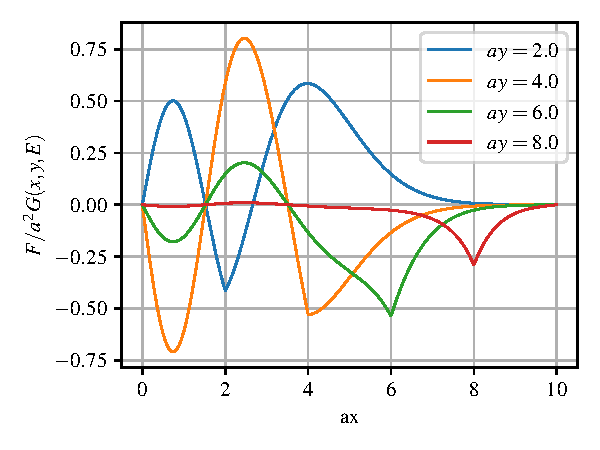
\includegraphics[scale=1]{./figs/1dgreens.pdf}
	\caption[Egy dimenziós Green-függvény]{}
	\label{egzakt:1dgreens}
\end{figure}

\begin{figure}[H]
	\centering
	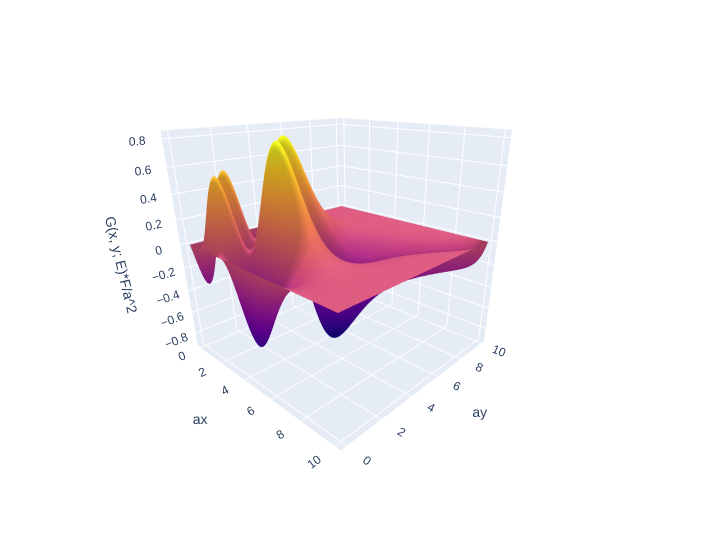
\includegraphics[scale=0.65]{./figs/2dgreen.png}
	\caption[Két dimenziós Green-függvény]{}
	\label{egzakt:2dgreen}
\end{figure}

\Aeqref{green:greensum} egyenletnek megfelelően a Green-függvénynek pólusai vannak $E=E_n$-ben. Ezt \aeqref{egzakt:greenfunction} egyértelmen mutatja, mivel a nevezőjében \aeqref{box_energiaszintek_egyenlet} $0$-ra rendezett egyenlet bal oldala szerepel. Ennek az egyenletnek a gykei határozták meg az $E_k$ sajátenergiákat.

Egy érdekes matematikai következmény, hogy a Green-függvényre vonatkozó differenciál egyenlet megoldásával elvégeztük \aref{green:greensum}. egyenlet összegzését. Ez az összeg az Airy függvények szorzatának összege lenne, osztva $E-E_k$-val és a megfelelő $N_k$ normálási faktorral ahol $E_k$-t \aeqref{box_energiaszintek_egyenlet} transzcendens egyenlet határoz meg. A Green-függvényre vonatkozó differenciálegyenlet ismerete nélkül az összeg elvégzése reménytelennek látszana.
	\subsection{Green-függvény határesetei}
		A két falú doboz Green-függvényéből megfelelő határesetekben előállítható más fizikai rendszerek Green-függvénye is. Például az $L\to\infty$ határeset visszaadja a felül nyitott doboz Green-függvényét, avagy a földön pattogó kvantum részecske ("quantum bouncer") Green-függvényét. Egy következő transzformáció határeseteként megkaphatjuk a falak nélküli végtelen lineáris potenciálban mozgó részecske Green-függvényét. Ehhez mind a helykoordinátát, mind az energiát meg kell változtatni: $x\to x^\prime=x+d$, $y\to y^\prime=y+d$ és $E\to E^\prime=E+Fd$, végül a $d\to\infty$ határesetet kell venni.

Az $L\to\infty$ határeset könnyen elvégezhető. \Aeqref{airy:ai+approx} és \aeqref{airy:bi+approx} egyenletek szerint $\Ti(aL-bE)$ gyorsan $0$-hoz tart. Ezt az eredményt felhasználva az $x=0$-ban fallal határolt részecske Green-függvénye $=Fx$ potenciálban
\begin{equation}
	G_{\text{egy fal}}\left(x,y;E\right) = -\frac{a^2}{F}\frac{\pi}{\Ti(-bE)}\times
	\begin{cases}
		\Ai(v)\Bigl(\Ti(-bE)\Bi(u)-\Ai(u)\Bigr)& x \leq y\\
		\Ai(u)\Bigl(\Ti(-bE)\Bi(v)-\Ai(v)\Bigr)& x \geq y
	\end{cases}.
	\label{limits:semiinfinite}
\end{equation}

A következő határesetet valamivel nehezebb kiszámítani. Ezt előre lehet sejteni, mert az eddigi Green-függvények olyan rendszereket írtak le, ahol minden állapot kötött állapot. A falak nélküli lineáris potenciálhoz nem tartoznak kötött állapotok, csak szórásállapotok vannak. Ez a változás megmutatkozik a Green-függvény pólusszerkezetében, utalva arra, hogy ez a határeset jelentősen megváltoztatja a Green-függvényt matematikai értelemben is. A feljebb említett átmenet,
\begin{equation}
	\begin{aligned}
		x^\prime&=x+d,\\
		y^\prime&=y+d,\\
		E^\prime&=E+Fd,\\
		d       &\to\infty.
	\end{aligned}
	\label{limits:transitiontonowall}
\end{equation}
E az átmenet eltolja a helykoordinátát, miközben a részecske kinetikus energiáját, változatlanul tartja. Az $u$ $v$ változók értéke \eqref{egzakt:uv} egyenlet szerint változatlan marad, a $d\to\infty$ határérték nem változtatja az alakjukat. Mivel a falak nélküli rendszernek az egész valós energiatengely a spektruma, a Green-függvényt az $E^\prime=E+Fd\pm i\epsilon$ energiában vizsgáljuk, a $\Ti(-bE^\prime)$ viselkedését kell meghatározni nagy $E^\prime$ esetén. Felhasználva \aeqref{airy:tiapprox} egyenletet
\begin{dmath}
	\Ti(-x-i\epsilon)
	\approx-\frac{\cos\left(\frac{2}{3}(x+i\epsilon)^{3/2}-\frac{\pi}{4}\right)}{\sin\left(x+i\epsilon)^{3/2}-\frac{\pi}{4}\right)}
	\approx-\frac{\cos\left(\frac{2}{3}x^{3/2}+i\sqrt{x}\epsilon-\frac{\pi}{4}\right)}{\sin\left(\frac{2}{3}x^{3/2}+i\sqrt{x}\epsilon-\frac{\pi}{4}\right)}
	=-\frac{\cos\left(\frac{2}{3}x^{3/2}-\frac{\pi}{4}\right)\cosh\left(\sqrt{x}\epsilon\right)-i\sin\left(\frac{2}{3}x^{3/2}-\frac{\pi}{4}\right)\sinh\left(\sqrt{x}\epsilon\right)}{\sin\left(\frac{2}{3}x^{3/2}-\frac{\pi}{4}\right)\cosh\left(\sqrt{x}\epsilon\right)+i\cos\left(\frac{2}{3}x^{3/2}-\frac{\pi}{4}\right)\sinh\left(\sqrt{x}\epsilon\right)}
	=-\frac{\cos\left(\frac{2}{3}x^{3/2}-\frac{\pi}{4}\right)-i\sin\left(\frac{2}{3}x^{3/2}-\frac{\pi}{4}\right)\tanh\left(\sqrt{x}\epsilon\right)}{\sin\left(\frac{2}{3}x^{3/2}-\frac{\pi}{4}\right)+i\cos\left(\frac{2}{3}x^{3/2}-\frac{\pi}{4}\right)\tanh\left(\sqrt{x}\epsilon\right)}
	\approx-\frac{\cos\left(\frac{2}{3}x^{3/2}-\frac{\pi}{4}\right)-i\sin\left(\frac{2}{3}x^{3/2}-\frac{\pi}{4}\right)\sgn\left(\epsilon\right)}{\sin\left(\frac{2}{3}x^{3/2}-\frac{\pi}{4}\right)+i\cos\left(\frac{2}{3}x^{3/2}-\frac{\pi}{4}\right)\sgn\left(\epsilon\right)}.
\end{dmath}
A sorok közötti lépésekhez felhasználtuk a $(x+a)^\alpha\approx x^\alpha + \alpha x^{\alpha-1}a$ közelítést, a trigonometrikus addíciós képleteket, a képzetes argumentumú trigonometrikus függvények és hiperbolikus függvények kapcsolatát, valamint az előel függvény közelítését a $\tanh$ függvénnyel. Ezek a közelítések egzaktak az $x\to\infty$ határesetben, ezért
\begin{equation}
	\lim_{x\to\infty}\Ti(-x-i\epsilon)=
	\begin{cases}
		i &\epsilon > 0\\
		-i&\epsilon < 0
	\end{cases}.
	\label{limits:ti}
\end{equation}
Ez az eredmény kellett ahhoz, hogy \aeqref{limits:transitiontonowall} átmenet alapján meghatározzuk a fal nélküli lineáris $V=Fx$ potenciálhoz tartozó Green-függényt. Ha $\Im(E)>0$
\begin{dmath}
	G_{\text{nincs fal}}(x,y;E)=\lim_{d\to\infty}G_{\text{egy fal}}(x+d,y+d;E+Fd)=\frac{\pi a^2}{F}\times
	\begin{cases}
		\Ai(v)\Bigl(\Bi(u)-i\Ai(u)\Bigr)&x\leq y\\
		\Ai(u)\Bigl(\Bi(v)-i\Ai(v)\Bigr)&x\geq y
	\end{cases}.
	\label{limits:nowallgreen1}
\end{dmath}
Ha $\Im(E)<0$, akkor \aeqref{limits:ti} egyenlet $-i$ a limeszben, így
\begin{dmath}
	G_{\text{nincs fal}}(x,y;E)=\lim_{d\to\infty}G_{\text{egy fal}}(x+d,y+d;E+Fd)=\frac{\pi a^2}{F}\times
	\begin{cases}
		\Ai(v)\Bigl(\Bi(u)+i\Ai(u)\Bigr)&x\leq y\\
		\Ai(u)\Bigl(\Bi(v)+i\Ai(v)\Bigr)&x\geq y
	\end{cases},
	\label{limits:nowallgreen2}
\end{dmath}
ez a kifejezés csak az $i$ előjelében különbözik az előzőtől. Az egész valós tengely mentén ugrása van ennek a Green-függvénynek a képzetes részének. Ez egybevág azzal a korábbi eredménnyel hogy tetszőleges energiájú sajátállapotai lehetnek a fal nélküli rendszernek, mert a Green-függvénynek vágása van a folytonos spektrumhoz tartozó energiák mentén.












	\subsection{Állapotsűrűség}
		Ahogy azt a Green-függvények bevezetésénél említettük, alkalmasak a (lokális) állapotsűrűség meghatározására \cite[7. o.]{economou2006green},
\begin{equation}
	\rho\left(E\right) = -\frac{1}{\pi}\lim_{\epsilon \to 0^+} \Im\Tr\op{G}\left(E + i\epsilon\right),
	\label{green:densityeq}
\end{equation}
\begin{equation}
	\rho(x,E)=-\frac{1}{\pi}\lim_{\epsilon\to 0^+}\Im G(x,x,E+i\epsilon).
	\label{green:localdensityeq}
\end{equation}
$\rho(E)\,dE$ az állapotok száma egy $dE$ energiatartományban, az állapotsűrűség. $\rho(x,E)\,dE\,dx$ pedig a megtalálási valószínűséggel súlyozott állapotok száma $dx$ intervallumban $dE$ energiatartományban, az úgynevezett lokális állapotsűrűség.

Ezeket a formulákat numerikus módon közelítőleg ki lehet értékelni kicsi, de véges $\epsilon$ választásával, ezt szemlélteti \aref{green:állapotsűrség}. ábra.
\begin{figure}[H]
	\centering
	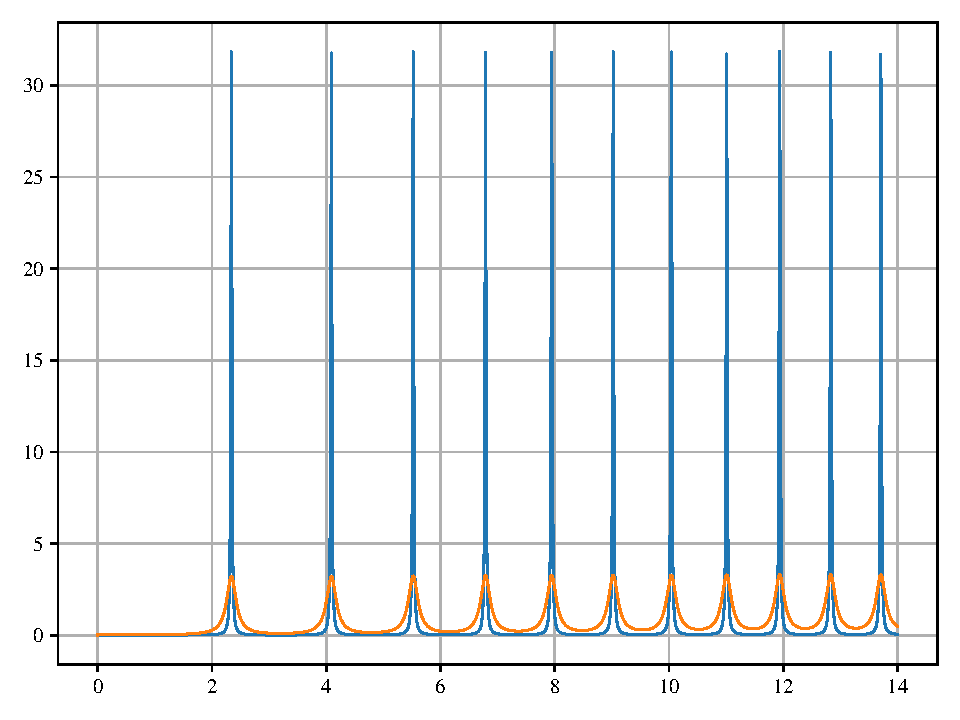
\includegraphics[scale=1]{./figs/dosfromgreen.pdf}
	\caption[Állapotsűrűség]{\Aref{green:densityeq}. képlet alapján számolt állapotsűrűség. A kék függvényt $\epsilon = 10^{-3}/b$, a narancssárga görbét pedig $\epsilon = 10^{-2}/b$ helyettesítéssel kaptuk. Látható, hogy $\epsilon$ csökkentésével a tüskék egyre keskenyebbek, és egyre magasabbak lesznek.}
	\label{green:állapotsűrség}
\end{figure}
Ennek a közelítésnek egy jó tulajdonsága, hogy a formula származtatásához a jól ismert
\begin{equation}
	\frac{1}{x\pm i\epsilon} = \frac{1}{x}\mp i\pi\delta(x)
\end{equation}
formulát lehet használni. Ennek a formulának a levezetése során a $\delta(x)$ állandó területű, de egyre szűkebb Lorentz-görbék határértékeként bukkan fel. Ez azt jelenti, hogy véges $\epsilon$ esetén is a sajátenergiákhoz tartozó csúcsok alatti terület változatlan, az állapotsűrűség $E$ szerinti integrálja nagy $E$-k és véges $\epsilon$ esetén is pontos marad.
\begin{figure}[H]
	\centering
	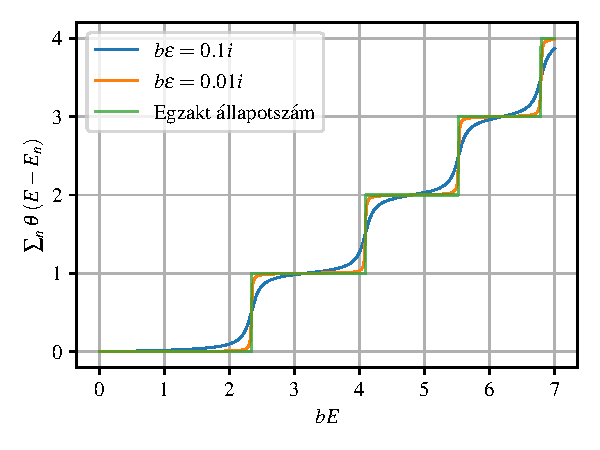
\includegraphics[scale=1]{./figs/numberofstatesfromgreen.pdf}
	\caption[Állapotok száma]{\Aref{green:állapotsűrség}. ábrán bemutatott függvények integrálja látható ezen az ábrán. Mind a két függvény ugrása közelítőleg $1$, ami at jelenti, hogy \aref{green:állapotsűrség}. ábrán látható tüskék alatti terület jó közelítéssel $1$. Az $\epsilon$ csökkentése a lépcsőfüggvényhez közelíti az integrált függvényt, ami egyezik az elvárásokkal.}
\end{figure}
\Aeqref{limits:semiinfinite} Green-függvényhez tartozó állapotsűrűség kvalitatíve nem különbözik az előző számítás menetétől és eredményétől, hiszen az előzőhöz hasonlóan csak diszkrét sajátenergiák vannak, ezeknek csupán az értékük különböző.

Más a helyzet \aeqref{limits:nowallgreen1}, \eqref{limits:nowallgreen2} Green-függvénnyel. Itt csak folytonos spektrumba tartozó sajátenergiák vannak, mind szórásállapotokhoz tartoznak. Ebben az esetben csak a lokális állapotsűrűséget lehet értelmezni, hiszen a sajátállapotok négyzetének integrálja végtelen, csak Dirac-deltára normálhatóak. \Aeqref{green:localdensityeq} egyenletnek megfelelően a határérték kiszámításához a pozitív képzetes részre vonatkozó \eqref{limits:nowallgreen1} kifejezést kell használni,
\begin{dmath}
	\rho(x,E)=-\frac{1}{\pi}\lim_{\epsilon\to 0^+}\Im\left\lbrace\frac{a^2\pi}{F}\Ai(ax-b(E+i\epsilon))\Bigl(\Bi(ax-b(E+i\epsilon))-i\Ai(ax-b(E+i\epsilon))\Bigr)\right\rbrace=\frac{a^2}{F}\Ai^2(ax-bE).
\end{dmath}
Nem meglepő módon ez az $E$ energiájú sajátállapot abszolútérték négyzete \eqref{nowell:sajátfüggvény}. A nomálási faktor is egyezik, hiszen $\frac{a^2}{F}=ab$.





















	\subsection{Perturbációszámítás}
		A perturbációszámításhoz a Hamilton operátort két részre bontom fel:
\begin{equation}
	\op{H} = \op{H}_0 + \op{V}
\end{equation}
A $\op{H}_0$ operátorhoz tartozó rezolvens $\op{G}_0\left(E\right)$. $\op{H}$ és $\op{H}_0$ kifejezhetőek a rezolvenseikkel. Ha a kifejezéseket behelyettesítjük a fenti egyenletbe, implicit egyenletet kapunk $op{G}\left(E\right)$-re nézve, melyet fel lehet használni perturbációszámításra. Az egyenletet balról $\op{G}_0^{-1}\left(E\right)$-vel, jobbról $\op{G}^{-1}\left(E\right)$-vel szorzunk.
\begin{equation}
	\op{G}^{-1}\left(E\right) + E = \op{G}_0^{-1}\left(E\right) + E + \op{V}
\end{equation}
\begin{equation}
	\op{G}\left(E\right) = \op{G}_0\left(E\right) - \op{G}_0\left(E\right)\op{V}\op{G}\left(E\right)
	\label{green:pertmaster}
\end{equation}
Az alábbi módon definiálva $\op{G}_n\left(E\right)$ operátort, \aref{green:pertmaster}. egyenlethez hasonló rekurziós összefüggés áll fent:
\begin{equation}
	\op{G}_n\left(E\right) = \op{G}_0\left(E\right)\sum_{k=0}^n\left(-\op{V}\op{G}_0\left(E\right)\right)^k
\end{equation}
\begin{equation}
	\op{G}_{n+1}\left(E\right) = \op{G}_0\left(E\right) - \op{G}_0\left(E\right)\op{V}\op{G}_n\left(E\right)
\end{equation}
Ha $\norm{\op{V}\op{G}_0\left(E\right)} < 1$ akkor a $\op{G}_n$ sorozat konvergál, és kielégíti \aref{green:pertmaster}. egyenletet. Ezért konvergencia esetén:
\begin{equation}
	\op{G}\left(E\right) = \op{G}_0\left(E\right)\sum_{n=0}^\infty\left(-\op{V}\op{G}_0\left(E\right)\right)^n
\end{equation}
A perturbbálatlan operátornak a lineáris potenciál nélküli dobozba zárt részecske Hamilton operátorát választom, $\op{H}_0=\frac{1}{2m}\op{p}^2$, így a lineáris potenciál marad a perturbáció $\op{V} = F\op{x}$. A perturbálatlan $\op{G}_0\left(E\right)$ Green-függvényt is \aref{green:Cbegin}-\ref{green:Cend}, \ref{green:xy}. és \aref{green:yx}. egyenletek alapján határozom meg.
\begin{equation}
	G_0\left(x,y;E\right) =
	\begin{cases}
		-\frac{2m}{k\hbar^2}\frac{1}{\sin\left(kL\right)} \sin\left(k\left(y-L\right)\right)\sin\left(kx\right) & x\leq y\\
		-\frac{2m}{k\hbar^2}\frac{1}{\sin\left(kL\right)} \sin\left(k\left(x-L\right)\right)\sin\left(ky\right) & x>y\\
	\end{cases}
\end{equation}
, ahol $k = \frac{\sqrt{2mE}}{\hbar}$.
\begin{figure}[H]
	\centering
	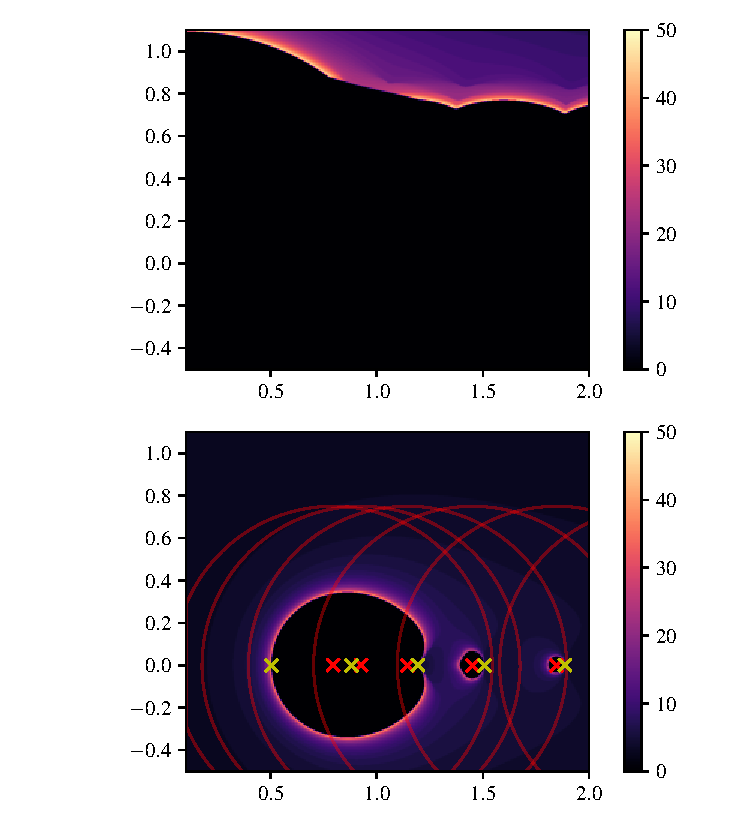
\includegraphics[scale=1]{./figs/convergence3.pdf}
	\caption[Green-függvény perturbációs sorának konvergenciája]{Ez az ábra a két perturbációs sor konvergenciáját hasonlítja össze a komplex energia síkon. A felső ábra a $V=Fx$ perturbáló potenciálnak, míg az alsó a $V = Fx-FL/2$ perturbáció szerinti sornak felel meg. A fekete tartományok divergenciát jelölnek, míg a többi szín a sorfejtés tagjainak csökkenési sebességét jellemzik, a norma harmadolásához szükséges lépések számát megadva. A piros körökön kívüli tartomány a ?? formula által garantált konvergencia tartományát jelöli. A piros x-ek a $\hat{G}_0$ pólusait, a sárga x-ek pedig az egzakt $\hat{G}$ operátor pólusait jelölik.}
\end{figure}
\section{Összegzés}
	A dolgozat első részében visszavezettük a háromdimenziós időfüggő problémát egydimenziós időfüggetlen problémákra, majd analitikus képleteket adtunk az egydimenziós probléma megoldásaira. Ezeket az egzakt képleteket összevetettük a szemiklasszikus közelítés eredményével, és a formulák fizikai interpretációját diszkutáltuk. Explicit analitikus képletet vezettünk le az időfüggetlen Green-függvényre, a pólusszerkezetét összevetettük az első részben kapott energiaszinteket meghatározó transzcendens egyenlettel. Szemléltettük a Green-függvény alkalmazhatóságát az állapotsűrűség numerikus illetve analitikus meghatározására is.

Egy konkrét példán bemutattuk, hogy a Hamiton-operátor önkényes felbontása perturbálatlan Hamilton-operátorra és perturbáló operátorra nagy mértékben befolyásolja a perturbációs sor konvergencia tulajdonságait. A példánkban a perturbáló operátor normájának minimalizálása egy triviális tag levonásával jelentősen javította a perturbációs sor konvergenciáját. Több részecske rendszereket leíró Green-függvények perturbációszámítása hatalmas jelentőséggel bír, számos fizikai témakör egyik fő eszköze, így a jövőben érdemes megvizsgálni, hogy milyen lehetőség van esetleg triviális tagok levonásával módosított perturbáció szerinti sorfejtés optimalizálására.
\appendix
\section{Szabad részecske gyorsuló koordinátarendszerben}
	Pozitív $x$ irányban 
\section{Numerikus számítások}
	\subsection{Momentumok időfejlődése}
		%\begin{figure}[H]
%	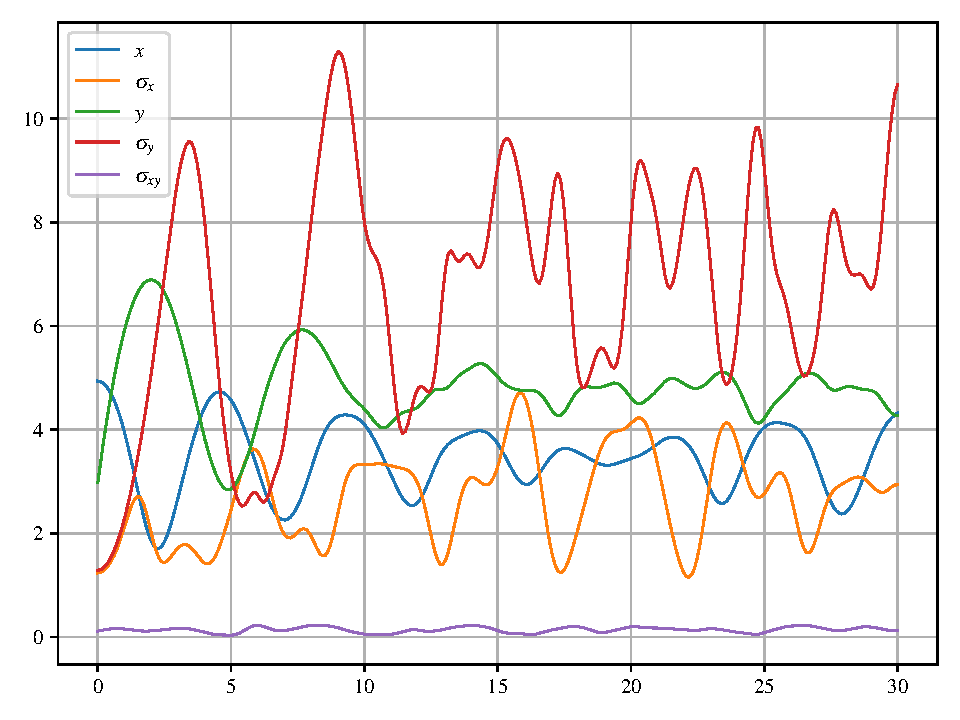
\includegraphics[scale=1]{./figs/expectations.pdf}
%	\caption{Várható értékek és szórások időfejlődése}
%\end{figure}

\begin{lstlisting}[language=Python]
def __init__(self, psi0 = None, F = 1.0, L = 15.0, numPoints = 200, name = "1D: "):
    self.__name = name
    self.__F = F
    self.__L = L
    self.__numPoints = numPoints
    self.__x = np.linspace(0, L, numPoints)
    
    self.__Es = np.zeros((0))
    self.__norms = np.zeros((0))
    self.__cachedBasisFun = np.zeros((0, self.__numPoints), dtype=complex)
    self.__c0s = np.zeros((0))
    
    if psi0 != None:
        self.__unormpsi0 = psi0
        self.__psi0norm = 1 / np.sqrt(np.abs(self.scalarProd(psi0, psi0)))
        n = 0
        while True:
            self.eLevel(n)
            self.waveFunNorm(n)
            self.cacheBasisFun(n)
            self.basisCoeff(n)
            
            eWaveFunSum = np.sum(np.abs(self.__c0s)**2)
            print(self.__name + "Sum of probabilities: " + str(eWaveFunSum))
            if eWaveFunSum > 0.9999:
                break
            n += 1
\end{lstlisting}

\begin{lstlisting}[language=Python]
def charEq(self, E, L = None):
    if L == None:
        L = self.__L
    F3sqrt = np.power(self.__F, 1/3)
    ai1, ai1p, bi1, bi1p = special.airy(-E / F3sqrt ** 2)
    ai1p /= F3sqrt ** 2
    bi1p /= F3sqrt ** 2
    ai2, ai2p, bi2, bi2p = special.airy(F3sqrt * L - E / F3sqrt ** 2)
    ai2p /= F3sqrt ** 2
    bi2p /= F3sqrt ** 2
    f = bi1*ai2 - ai1*bi2
    fp = -(bi1p*ai2 + bi1*ai2p - (ai1p*bi2 + ai1*bi2p))
    return f, fp
\end{lstlisting}

\begin{lstlisting}[language=Python]
def eLevel(self, n):
    '''
    n goes from 0
    '''
    if len(self.__Es) <= n:
        for i in range(len(self.__Es), n+1):
            lstart = 1 / np.power(self.__F, 1/3)
            if self.__L <= lstart:
                llist = np.array([self.__L])
                stepsize = float("nan")
            else:
                stepsize = 0.1
                stepnum = int((self.__L-lstart)//stepsize) + 1
                stepsize = (self.__L-lstart)/stepnum
                llist = np.linspace(lstart, self.__L, stepnum+1)
            Eguess = (np.pi * (i+1) / llist[0]) ** 2
            E = 0
            for l in llist:
                E = (optimize.root_scalar(f=self.charEq, args = (l), x0=Eguess, fprime=True)).root
                Eguess = E * (l/(l+stepsize))**2
            print(self.__name + f"E_{i:d}={E:.2f}")
            self.__Es = np.append(self.__Es, E)
    return
\end{lstlisting}

\begin{lstlisting}[language=Python]
def unormWaveFun(self, x, n):
    '''
    n goes from 0
    '''
    self.eLevel(n)
    E = self.__Es[n]
    F3sqrt = np.power(self.__F, 1/3)
    ai1, ai1p, bi1, bi1p = special.airy(-E / F3sqrt ** 2)
    ai2, ai2p, bi2, bi2p = special.airy(F3sqrt * x - E / F3sqrt ** 2)
    mask = np.array(E / F3sqrt ** 2 - F3sqrt * x > -10).astype(float)
    return (bi1 * ai2 - ai1 * bi2) * mask
\end{lstlisting}

\begin{lstlisting}[language=Python]
def waveFunNorm(self, n):
    '''
    n goes from 0
    '''
    F3sqrt = np.power(self.F, 1/3)
    if len(self.__norms) <= n:
        for i in range(len(self.__norms), n+1):
            self.eLevel(i)
            ai1, ai1p, bi1, bi1p = special.airy(-self.Es[i] / F3sqrt**2)
            ai2, ai2p, bi2, bi2p = special.airy(self.L * F3sqrt - self.Es[i] / F3sqrt**2)
            intsquared = 1 / F3sqrt * (1 / np.pi**2 - (bi1*ai2p - ai1*bi2p * (self.Es[i] - self.L * self.F > -10))**2)
            norm = 1 / np.sqrt(intsquared)
            print(self.__name + f"N_{i:d}={norm:.2f}")
            self.__norms = np.append(self.__norms, norm)
    return
\end{lstlisting}

\begin{lstlisting}[language=Python]
def scalarProd(self, a, b):
    real = integrate.quad(lambda x: np.real(np.conjugate(a(x)) * b(x)), 0, self.__L)[0]
    imag = integrate.quad(lambda x: np.imag(np.conjugate(a(x)) * b(x)), 0, self.__L)[0]
    return real + 1j * imag
\end{lstlisting}

\begin{lstlisting}[language=Python]
def G(self, x, y, E):
    F3sqrt = np.power(self.__F, 1/3)
    ai1, ai1p, bi1, bi1p = special.airy(-E / F3sqrt**2)
    ai2, ai2p, bi2, bi2p = special.airy((self.__F * self.__L - E) / F3sqrt**2)
    ai3, ai3p, bi3, bi3p = special.airy(x * F3sqrt - E / F3sqrt**2)
    ai4, ai4p, bi4, bi4p = special.airy(y * F3sqrt - E / F3sqrt**2)
    c0 = 1 / F3sqrt * np.pi / (ai1/bi1 - ai2/bi2)
    G1 = c0 * (ai4 - ai2/bi2 * bi4) * (ai3 - ai1/bi1 * bi3) * (x < y)
    G2 = c0 * (ai4 - ai1/bi1 * bi4) * (ai3 - ai2/bi2 * bi3) * (1 - (x < y))
    return G1 + G2
\end{lstlisting}

\begin{lstlisting}[language=Python]
def timeEvolution(self, t = 0):
    ret = np.zeros((self.__numPoints), dtype = complex)
    for n in range(len(self.__cachedBasisFun)):
        ret += self.__c0s[n] * np.exp(-1j * self.__Es[n]*t) * self.__cachedBasisFun[n, :]
    return ret
\end{lstlisting}

\begin{lstlisting}[language=Python]
def G(self, x, y, E):
    F3sqrt = np.power(self.__F, 1/3)
    ai1, ai1p, bi1, bi1p = special.airy(-E / F3sqrt**2)
    ai2, ai2p, bi2, bi2p = special.airy((self.__F * self.__L - E) / F3sqrt**2)
    ai3, ai3p, bi3, bi3p = special.airy(x * F3sqrt - E / F3sqrt**2)
    ai4, ai4p, bi4, bi4p = special.airy(y * F3sqrt - E / F3sqrt**2)
    c0 = 1 / F3sqrt * np.pi / (ai1/bi1 - ai2/bi2)
    G1 = c0 * (ai4 - ai2/bi2 * bi4) * (ai3 - ai1/bi1 * bi3) * (x < y)
    G2 = c0 * (ai4 - ai1/bi1 * bi4) * (ai3 - ai2/bi2 * bi3) * (1 - (x < y))
    return G1 + G2
\end{lstlisting}

\begin{lstlisting}[language=Python]
test = d1schroedinger(L=7)

def convergence(E):
    G0 = test.G0(x, y, E)
    VG0 = test.F * x * G0 / N * test.L
    realG = test.G(x, y, E)
    G = G0
    norm0 = dx * np.linalg.norm(G0 @ VG0, ord=2)
    norms = np.array([norm0])
    steps = np.array([0])
    for i in range(20):
        G = G0 + G @ VG0
        norm = dx * np.linalg.norm(G - realG, ord=2)
        norms = np.append(norms, norm)
        steps = np.append(steps, i+1)
        if norm/norm0 + norm0/norm > 5:
            break
    
    popt, pcov = curve_fit(normguess, steps, norms/norms[0])
    return -popt[0]
\end{lstlisting}
	\subsection{Hullámfüggvény időfejlődése}
		\subsubsection{1D}
		\subsubsection{2D}
	
    \newpage
	\phantomsection
	\bibliographystyle{abeld}
	\addcontentsline{toc}{section}{Hivatkozások}
    \bibliography{tex/ref}
\end{document}















